% final Aug 8 2018
% pre-final  Aug 6 2018
% Frank.Nielsen@acm.org July 3rd 2018
\documentclass[graybox]{svmult}

 

\usepackage{times,amssymb,url,amsmath,graphicx,ifpdf,booktabs,bm}
\usepackage[ruled,vlined,linesnumbered,lined]{algorithm2e}
\usepackage[justification=centering]{caption}
\usepackage{subcaption}
\captionsetup{compatibility=false}

\usepackage{multirow}
\usepackage{amsmath,amssymb}

\usepackage{mathptmx}       % selects Times Roman as basic font
\usepackage{helvet}         % selects Helvetica as sans-serif font
\usepackage{courier}        % selects Courier as typewriter font
\usepackage{type1cm}        % activate if the above 3 fonts are
                            % not available on your system
%
\usepackage{makeidx}         % allows index generation
\usepackage{graphicx}        % standard LaTeX graphics tool
                             % when including figure files
\usepackage{multicol}        % used for the two-column index
\usepackage[bottom]{footmisc}% places footnotes at page bottom

 

\makeindex             % used for the subject index
                       % please use the style svind.ist with
                       % your makeindex program

%%%%%%%%%%%%%%%%%%%%%%%%%%%%%%%%%%%%%%%%%%%%%%%%%%%%%%%%%%%%%%%%%%%%%%%%%%%%%%%%%%%%%%%%%


 
	
\graphicspath{{./figures/}}
\ifpdf \DeclareGraphicsRule{*}{mps}{*}{} \fi

\sloppy

\def\eps{\epsilon}
% identity function
\def\sign{\mathrm{sign}}
\def\idf{\mathrm{id}}
\def\CS{\mathrm{CS}}
\def\LC{\mathrm{LC}}
\def\KL{\mathrm{KL}}
\def\tr{\mathrm{tr}}
\def\dnu{\mathrm{d}\nu}
\def\dt{\mathrm{d}t}
\def\dx{\mathrm{d}x}
\def\dy{\mathrm{d}y}
\def\calB{\mathcal{B}}
\def\calM{\mathcal{M}}
\def\calH{\mathcal{H}}
\def\calI{\mathcal{I}}
\def\calX{\mathcal{X}}
\def\calC{\mathcal{C}}
\def\calD{\mathcal{D}}
\def\calF{\mathcal{F}}
\def\calV{\mathcal{V}}
\def\tp{\tilde{p}}
\def\tq{\tilde{q}}
\def\bbR{\mathbb{R}}
\def\Finner#1#2#3{{\langle {#1},\;{#2} \rangle}_{#3}}
\def\inner#1#2{ \langle {#1},{#2} \rangle }

\def\Bhat{\mathrm{Bhat}}
\def\Holder{\mathrm{H}}
\def\JB{\mathrm{JB}}

\def\aff{\mathrm{affine}}
\def\co{\mathrm{hull}}
\DeclareMathOperator*{\argmax}{arg\,max}
\DeclareMathOperator*{\argmin}{arg\,min}
\def\st{\ :\ } 

\def\FHR{\mathrm{FHR}}
\def\IG{\mathrm{IG}}
\def\HG{\mathrm{HG}}
\def\NH{\mathrm{NH}}  % Normed Hilbert

\def\dP{{\mathrm{d}P}}
\def\dQ{{\mathrm{d}Q}}

\begin{document}

\title*{Clustering in Hilbert Geometry\\{Two Case Studies: The Probability Simplex and the Correlation Elliptope}}
\titlerunning{Clustering in Hilbert Geometry}
 
\author{Frank Nielsen \and Ke Sun}
\authorrunning{Nielsen Sun}
\institute{Frank Nielsen \at Sony Computer Science Laboratories, Tokyo, Japan,
\email{Frank.Nielsen@acm.org}
\and Ke Sun \at CSIRO Data61, Sydney, Australia,
\email{Ke.Sun@data61.csiro.au}}

\maketitle

\abstract{
Clustering categorical distributions in the probability simplex is a fundamental primitive often met in applications
dealing with histograms or mixtures of multinomials.
Traditionally, the differential-geometric structure of the probability simplex has been used either by
(i) setting the Riemannian metric tensor to the Fisher information matrix of the categorical distributions, or
(ii) defining the information-geometric structure induced by a smooth dissimilarity measure, called a divergence.
In this work, we introduce a novel computationally-friendly non-differential framework for modeling the probability simplex: Hilbert simplex geometry.
We discuss the pros and cons of those three statistical modelings, and compare them experimentally for clustering tasks. 
}

\noindent Keywords: Fisher-Riemannian geometry, information geometry,  Hilbert simplex geometry, Finsler geometry, center-based clustering.



%%%%%%%%%%
\section{Introduction}\label{sec:intro}
%%%%%%%%%%

The multinomial distribution is an important representation in machine learning that is often met
in applications~\cite{MetricLearning-2002, ClusteringSimplex-2008} as normalized histograms (with non-empty bins). 
A multinomial distribution (or categorical distribution) $p\in\Delta^d$ can be thought as a point lying in the probability simplex $\Delta^d$ (standard simplex) with coordinates $p=(\lambda_p^0,\ldots,\lambda_p^d)$ such that $\lambda_p^i>0$ and $\sum_{i=0}^d \lambda_p^i=1$.
The open probability simplex $\Delta^d$ sits in $\bbR^{d+1}$ on the hyperplane $H_{\Delta^d}:\;\sum_{i=0}^d x^i =1$.
We consider the task of clustering a set $\Lambda=\{p_1,\ldots,p_n\}$ of $n$ categorical distributions
in $\Delta^d$~\cite{ClusteringSimplex-2008}
using center-based $k$-means++ or $k$-center clustering algorithms~\cite{kmeanspp-2007,kcenter-1985},
which rely on a dissimilarity measure (loosely called distance or divergence when smooth) between any two categorical distributions. 
In this work, we mainly consider three distances with their underlying geometries:
(1) Fisher-Hotelling-Rao distance $\rho_\FHR$, (2) Kullback-Leibler divergence $\rho_\IG$, and (3) Hilbert distance $\rho_\HG$.
The geometric structures are necessary in algorithms, for example, to define midpoint distributions.
Figure~\ref{fig:results} displays the $k$-center clustering results obtained with these three geometries
as well as the Euclidean $L^1$ distance $\rho_{L1}$ on toy datasets in $\Delta^2$.
We shall now explain the Hilbert simplex geometry applied to the probability simplex, describe
how to perform $k$-center clustering in Hilbert geometry, and report experimental results that
demonstrate superiority of the Hilbert geometry when clustering multinomials.

\begin{figure*}[!t]
\centering
\begin{subfigure}{\textwidth}
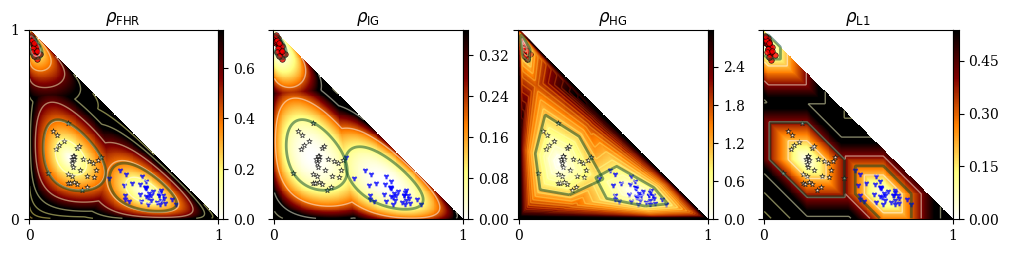
\includegraphics[width=\textwidth]{kcenters3}
\caption{$k=3$ clusters}
\end{subfigure}
\begin{subfigure}{\textwidth}
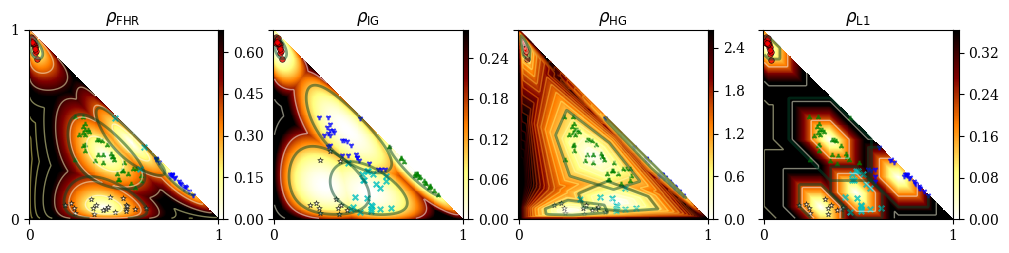
\includegraphics[width=\textwidth]{kcenters5}
\caption{$k=5$ clusters}
\end{subfigure}
\caption{$k$-Center clustering results on a toy dataset in the space of trinomials $\Delta^2$.
The color density maps indicate the distance from any point to its nearest cluster center.}\label{fig:results}
\end{figure*}

The rest of this paper is organized as follows:
Section~\ref{sec:distances} formally introduces the distance measures in $\Delta^d$.
Section~\ref{sec:dist} introduces how to efficiently compute the Hilbert distance.
Section~\ref{sec:clustering} presents algorithms for Hilbert minimax centers and Hilbert clustering.
Section~\ref{sec:exp} performs an empirical study of clustering multinomial distributions,
comparing Riemannian geometry, information geometry and Hilbert geometry.
Section~\ref{sec:elliptope} presents a second use case of Hilbert geometry in machine learning:
clustering correlation matrices.
Finally, section~\ref{sec:con} concludes this work by summarizing the pros and cons of each geometry.
Although some contents require prior knowledge on geometric structures, 
we will present the detailed algorithms so that general audience can still benefit from this work.

%%%%%%%%%%%%%%%%%%%%%%%%%%%%%%%%%%%%%%%%%%%%%%%%%%%%%%%%%%%%
\section{Three distances with their underlying geometries}\label{sec:distances}
%%%%%%%%%%%%%%%%%%%%%%%%%%%%%%%%%%%%%%%%%%%%%%%%%%%%%%%%%%%%

\subsection{Fisher-Hotelling-Rao geometry}

The Rao distance between two multinomial distributions is~\cite{KassVos-1997,MetricLearning-2002}:
\begin{equation}
\rho_{\FHR}(p,q) = 2\arccos\left(\sum_{i=0}^{d} \sqrt{\lambda_p^i\lambda_q^i}\right).
\end{equation}
It is a Riemannian metric length distance (satisfying the symmetric and triangular inequality axioms)
obtained by setting the metric tensor $g$ to the {\em Fisher information matrix} (FIM)
$\mathcal{I}(p)=(g_{ij}(p))_{d\times{d}}$ wrt the coordinate system $(\lambda_p^1,\cdots,\lambda_p^d)$,
where
$$
g_{ij}(p) = \frac{\delta_{ij}}{\lambda_p^i} + \frac{1}{\lambda_p^0}.
$$
We term this geometry the Fisher-Hotelling-Rao (FHR) geometry~\cite{Hotelling-1930,storyLM-2007,Rao-1945,Rao-reprint-1992}.
The metric tensor $g$ allows to define an inner product on each tangent plane $T_p$ of the probability simplex manifold: $\Finner{u}{v}{p}=u^\top g(p) v$.
When $g$ is everywhere the identity matrix, we recover the Euclidean (Riemannian) geometry with the inner product being the scalar product: $\inner{u}{v}=u^\top v$.
The geodesics $\gamma(p,q;\alpha)$ are defined by the Levi-Civita metric connection~\cite{IG-2016,IG-2014}.
The FHR manifold can be embedded in the positive orthant of an Euclidean $d$-sphere in $\bbR^{d+1}$
by using the {\em square root representation} $\lambda\mapsto\sqrt{\lambda}$~\cite{KassVos-1997}.
Therefore the FHR manifold modeling of $\Delta^d$ has constant {\em positive} curvature: It is a
spherical geometry restricted to the positive orthant with the metric distance measuring the arc length on a great circle.

%%%%%%%%%%%%%
\subsection{Information geometry}
%%%%%%%%%%%%%%

A divergence $D$ is a smooth $C^3$ differentiable dissimilarity measure~\cite{DivIG-2010}
that allows to define a dual structure in Information Geometry~(IG;\;\cite{HessianStructure-2007,IG-2014,IG-2016}).
A $f$-divergence is defined for a strictly convex function $f$ with $f(1)=0$ by:
$$
I_f(p:q)=\sum_{i=0}^{d} \lambda_p^i f\left(\frac{\lambda_q^i}{\lambda_p^i}\right). 
$$
It is a {\em separable} divergence since the $d$-variate divergence can be written as a sum of $d$ univariate divergences: 
$I_f(p:q)=\sum_{i=0}^{d} I_f( \lambda_p^i: \lambda_q^i)$.
The class of $f$-divergences plays an essential role in information theory since they are provably the {\em only} separable divergences that satisfy
 the {\em information monotonicity} property~\cite{IG-2016,SeparableDivergence-2016}. 
That is, by coarse-graining the histograms  
we obtain lower-dimensional multinomials, say $p'$ and $q'$, such that $0\leq I_f(p':q')\leq  I_f(p:q)$~\cite{IG-2016}.
The Kullback-Leibler (KL) divergence $\rho_{\IG}$ is a $f$-divergence obtained for $f(u)=-\log u$:
\begin{equation}
\rho_{\IG}(p,q) = \sum_{i=0}^d \lambda_p^i \log\frac{\lambda_p^i}{\lambda_q^i}.
\end{equation}
It is an asymmetric non-metric distance: $\rho_{\IG}(p,q)\not =\rho_{\IG}(q,p)$.
In differential geometry, the structure of a manifold is defined by two components: 
\begin{enumerate}
\item A {\em metric tensor} $g$ that allows to define an inner product $\Finner{\cdot}{\cdot}{p}$ at each tangent space (for measuring vector lengths and angles between vectors); 
\item A {\em connection} $\nabla$ that defines 
{\em parallel transport} $\prod_{p,q}^\nabla$, {\it i.e.}, a way to move a tangent vector from
one tangent plane $T_p$ to any other one $T_q$.
\end{enumerate}
In FHR geometry, the implicitly-used connection is called the Levi-Civita connection that is induced by the metric $g$: $\nabla^{LC}=\nabla(g)$.
It is a metric connection since it ensures that $\Finner{u}{v}{p}=\Finner{\prod_{p,q}^{\nabla^\LC} u}{\prod_{p,q}^{\nabla^\LC} v}{q}$. 
The underlying information-geometric structure of KL is characterized by a pair of \emph{dual} connections~\cite{IG-2016} 
$\nabla=\nabla^{(-1)}$ (mixture connection) and $\nabla^*=\nabla^{(1)}$ (exponential connection) that induces a corresponding pair of dual geodesics
(technically, $\pm1$-autoparallel curves,~\cite{IG-2014}). Those connections are said \emph{flat} as they define two dual affine
coordinate systems $\theta$ and $\eta$ on which the $\theta$- and $\eta$-geodesics are straight line segments, respectively. 
For multinomials, the {\em expectation parameters} are: $\eta = (\lambda^1,\ldots,\lambda^d)$
and they one-to-one correspond to the {\em natural parameters}:
$\theta = \left(\log\frac{\lambda^1}{\lambda^0},\ldots,\log\frac{\lambda^d}{\lambda^0}\right)$.
Thus in IG, we have two kinds of midpoint multinomials of $p$ and $q$, depending on whether we perform the (linear) interpolation
on the $\theta$- or the $\eta$-geodesics.
Informally speaking, the dual connections $\nabla^{(\pm 1)}$ are said coupled to the FIM since we have  
$\frac{\nabla+\nabla^*}{2}=\nabla(g)=\nabla^{\LC}$. Those dual connections are not metric connections but enjoy the following property:
$\Finner{u}{v}{p} = \Finner{{\prod}_{p,q} u}{{\prod^*}_{p,q} v}{q}$, where $\prod=\prod^{\nabla}$ and ${\prod^*}={\prod^{\nabla^*}}$
are the corresponding induced dual parallel transports.
The geometry of $f$-divergences~\cite{DivIG-2010} is the $\alpha$-geometry (for $\alpha=3+2f'''(1)$) with the dual $\pm\alpha$-connections,
where $\nabla^{(\alpha)}=\frac{1+\alpha}{2}\nabla^*+\frac{1-\alpha}{2}\nabla$. The Levi-Civita metric connection is $\nabla^\LC=\nabla^{(0)}$.
More generally, it was shown how to build a dual information-geometric structure for {\em any} divergence~\cite{DivIG-2010}.
For example, we can build a dual structure from the symmetric Cauchy-Schwarz divergence~\cite{CS-2006}:
\begin{equation}
\rho_\CS(p,q)=- \log \frac{\inner{\lambda_p}{\lambda_q}}{\sqrt{\inner{\lambda_p}{\lambda_p}\inner{\lambda_q}{\lambda_q}}}.
\end{equation}

 %%%%%%%%%%%%
\subsection{Hilbert simplex geometry}
%%%%%%%%%%%%

\begin{figure}%
\centering%
\includegraphics[width=.4\textwidth]{hg.1}%
\caption{Computing the Hilbert distance for trinomials on the 2D probability simplex.}%
\label{fig:hd}%
\end{figure}

In Hilbert geometry~(HG; \cite{Hilbert-1895}), we are given a bounded convex domain $\calC$ (here, $\calC=\Delta^d$),
and the distance between any two points $M$, $M'$ of $\calC$ is defined as follows:
Consider the two intersection points $AA'$ of the line $(MM')$ with  $\calC$, and order them on the line so that we have $A,M,M',A'$. 
Then the Hilbert metric distance~\cite{Busemann-2011} is defined by:
\begin{equation}\label{eg:hgd}
\rho_{\mathrm{HG}}(M,M')=\left\{
\begin{array}{ll}
\left\vert\log\frac{|A'M| |AM'|}{|A'M'| |AM|}\right\vert, & M \not=M',\\
0 & M=M'.
\end{array}
\right.
\end{equation}
It is also called the Hilbert cross-ratio metric distance~\cite{HilbertHarpe-1991,BH-2014}.
Notice that we take the absolute value of the logarithm since the Hilbert distance is a {\em signed distance}~\cite{Richter-2011}.
When $\calC$ is the unit ball, HG lets us recover the Klein hyperbolic geometry~\cite{BH-2014}.
When $\calC$ is a quadric bounded convex domain, we obtain the Cayley-Klein hyperbolic geometry~\cite{CKM-2015}
which can be studied with the Riemannian structure and the corresponding metric distance called the curved Mahalanobis
distances~\cite{LMNN-2016,CayleyClassification-2016}.
Cayley-Klein hyperbolic geometries have negative curvature.

In Hilbert geometry, the geodesics are {\em straight} Euclidean lines making them convenient for computation.
Furthermore, the domain boundary $\partial\calC$ needs not to be smooth: One may also consider bounded polytopes~\cite{HGPolytope-2009}.
This is particularly interesting for modeling $\Delta^d$, the $d$-dimensional open standard simplex.
We call this geometry the \emph{Hilbert simplex geometry}.
In Figure~\ref{fig:hd}, we show that the Hilbert distance between two multinomial distributions
$p$ ($M$) and $q$ ($M'$) can be computed by
finding the two intersection points of the line $(1-t)p+tq$ with
$\partial\Delta^d$, denoted as $t_0\le0$ and $t_1\ge1$. Then 
$$
\rho_{\mathrm{HG}}(p,q)=\left\vert\log\frac{(1-t_0)t_1}{(-t_0)(t_1-1)}\right\vert
=\log\left(1-\frac{1}{t_0}\right)-\log\left(1-\frac{1}{t_1}\right).
$$

\begin{figure}[t]%
\centering
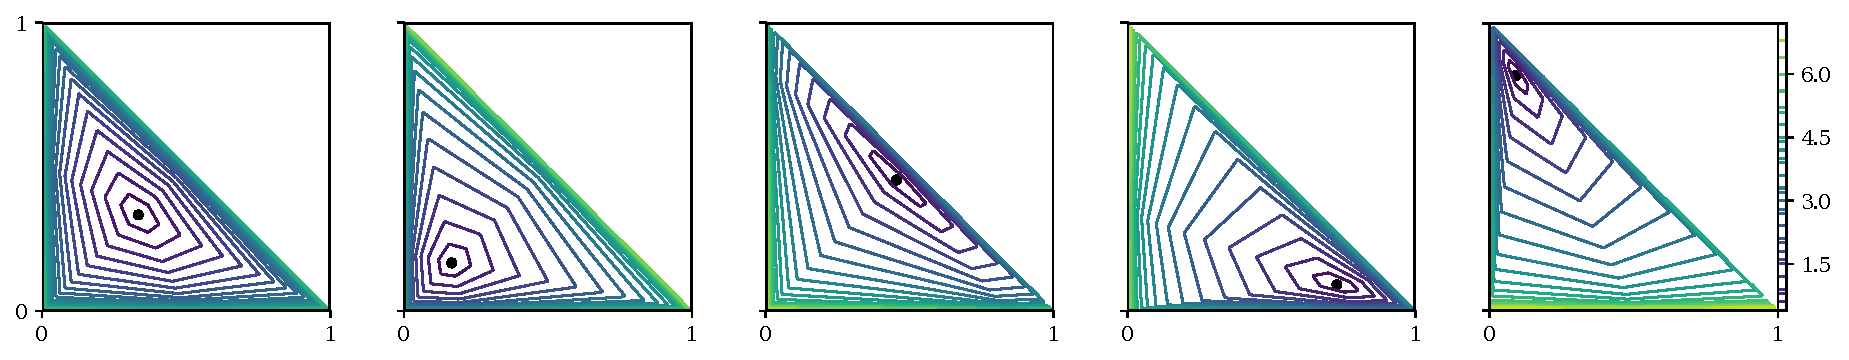
\includegraphics[width=\textwidth]{ball}
\caption{Balls in the  Hilbert simplex geometry $\Delta^2$ have polygonal Euclidean shapes of constant combinatorial complexity.
At infinitesimal scale, the balls have hexagonal shapes, showing that the Hilbert geometry is not Riemannian.}%
\label{fig:shape}%
\end{figure}

\begin{figure}
\centering
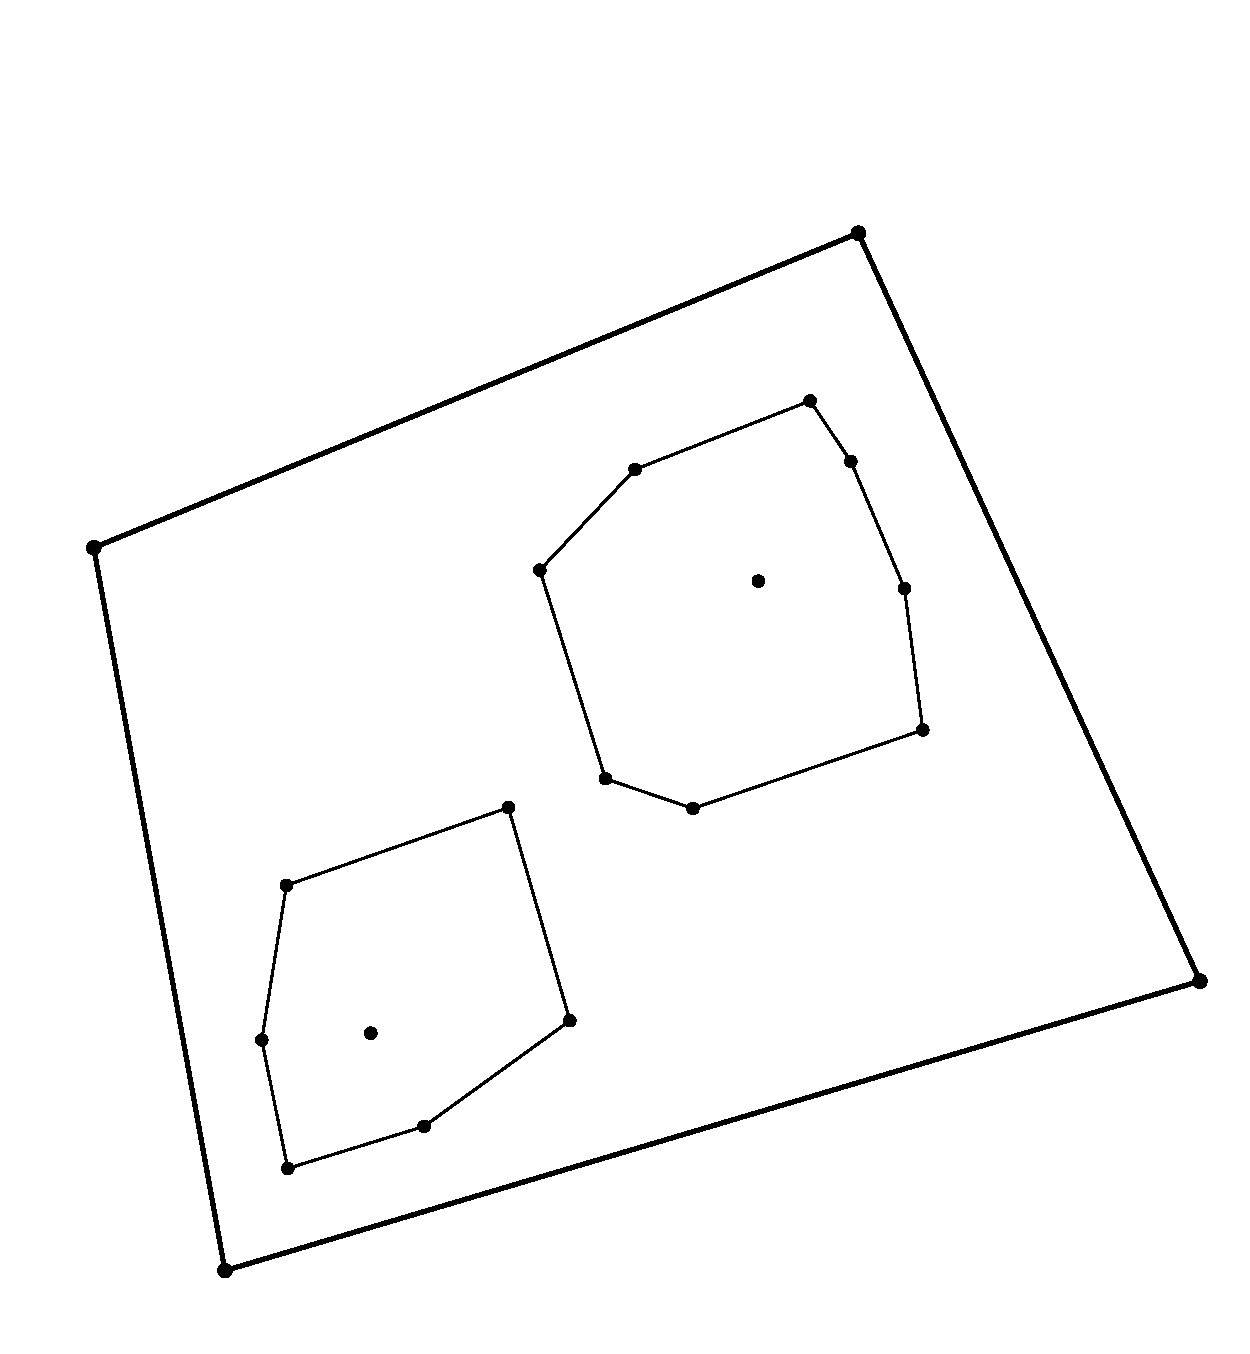
\includegraphics[width=.25\textwidth]{quadrangle}\hskip 3cm
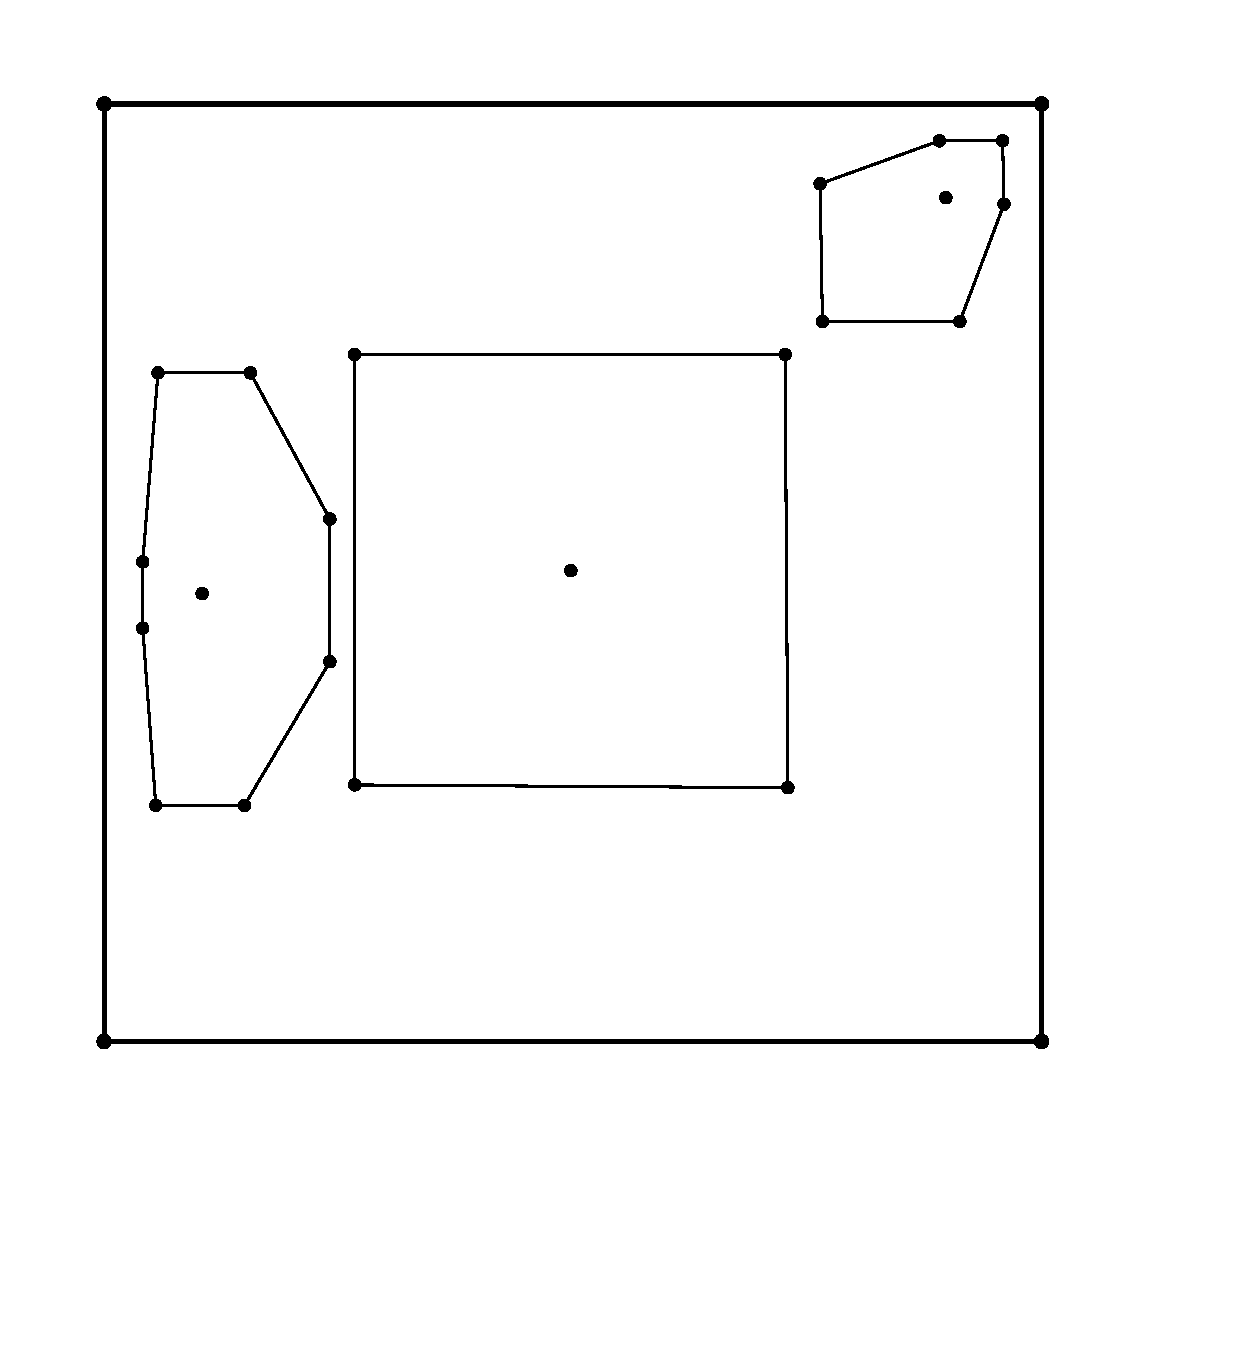
\includegraphics[width=.25\textwidth]{square}
\caption{Hilbert Balls in quadrangle domains have combinatorial complexity depending on the center location.\label{fig:quad}}
\end{figure}



The shape of balls in polytope-domain HG is Euclidean polytopes~\cite{BH-2014},
as depicted in Figure~\ref{fig:shape}.
Furthermore, the Euclidean shape of the balls do not change with the radius.
Hilbert balls have hexagons shapes in 2D~\cite{HG-SoCG-2017}, rhombic dodecahedra shapes in 3D, and are polytopes~\cite{BH-2014} with $d(d+1)$ facets in dimension $d$.
When the polytope domain is not a simplex, the combinatorial complexity of balls depends on the center location~\cite{HG-SoCG-2017}, see Figure~\ref{fig:quad}.
The HG of the probability simplex yields a non-Riemannian geometry, because at infinitesimal radius, the balls are polytopes and not ellipsoids
(corresponding to squared Mahalanobis distance balls used to visualize metric tensors \cite{VizTensor-2009}).
The isometries in Hilbert polyhedral geometries are studied in~\cite{HilbertIsometry-2011}.
In Appendix~\ref{sec:HGFG}, we recall that any Hilbert geometry induces a Finslerian structure
that becomes Riemannian iff the boundary is an ellipsoid (yielding the hyperbolic Cayley-Klein geometries~\cite{Richter-2011}).
Notice that in Hilbert simplex/polytope geometry, the geodesics are not unique (see Figure~2 of~\cite{HilbertHarpe-1991}).

\begin{table*}[t]
\centering
\caption{Comparing the three geometric modelings of the probability simplex $\Delta^d$.}\label{tab:geo}

{\small
\begin{tabular}{rlll}
\toprule[1.5pt]
 & {\bf{Riemannian Geometry}} & {\bf{Information Rie. Geo.}} & {\bf{Non-Rie. Hilbert Geo.}}\\\hline
Structure & $(\Delta^d,g,\nabla^\LC=\nabla(g))$ & $$ $(\Delta^d,g,\nabla^{(\alpha)},\nabla^{(-\alpha)})$ & $(\Delta^d,\rho)$\\  %  or $(\Delta^d,g,T)$
 & Levi-Civita $\nabla^\LC=\nabla^{(0)}$  & dual connections $\nabla^{(\pm\alpha)}$ so & connection of $\bbR^d$\\
 & &  that $\frac{\nabla^{(\alpha)} + \nabla^{(-\alpha)}}{2}=\nabla^{(0)}$  & \\
Distance & Rao distance (metric) & $\alpha$-divergence (non-metric) & Hilbert distance (metric)\\
 & & KL or reverse KL for $\alpha=\pm1$\\
Property & invariant to reparameterization & information monotonicity & isometric to a normed space \\
Calculation & 
closed-form & closed-form & easy (Alg. 1)\\
Geodesic & shortest path & straight either in $\theta/\eta$ & straight\\
Smoothness & manifold  & manifold & non-manifold\\
Curvature & positive & dually flat & negative\\
\bottomrule[1.5pt]
\end{tabular}}
\end{table*}

Table~\ref{tab:geo} summarizes the characteristics of the three introduced geometries: FHR, IG, and HG.
Let us conclude this introduction by mentioning the Cram\'er-Rao lower bound and its relationship with information geometry~\cite{CRLB-2013}:
Consider an unbiased estimator $\hat\theta=T(X)$ of a parameter $\theta$ estimated from
measurements distributed according to a smooth density $p(x;\,\theta)$ (i.e., $X\sim{p}(x;\,\theta)$).
The Cram\'er-Rao Lower Bound (CRLB) states that the variance of $T(X)$ is greater or equal to the inverse of the FIM $\calI(\theta)$:
$V_\theta[T(X)]\succ\calI^{-1}(\theta)$. For regular parametric families $\{p(x;\theta)\}_\theta$, the FIM is a positive-definite matrix and defines a metric tensor, called the Fisher metric in Riemannian geometry. The FIM is the cornerstone of information geometry~\cite{IG-2016} but requires the differentiability of the probability density function (pdf).

A better lower bound that does not require the pdf differentiability is the Hammersley-Chapman-Robbins Lower Bound~\cite{Hammersley-1950,ChapmanRobbins-1951} (HCRLB):
\begin{equation}
V_\theta[T(X)]\geq \sup_\Delta \frac{\Delta^2}{E_\theta\left[\left(\frac{p(x;\theta+\Delta)-p(x;\theta)}{p(x;\theta)}\right)^2\right]}.
\end{equation}
By introducing the $\chi^2$-divergence, $\chi^2(P:Q)=\int \left(\frac{\dP-\dQ}{\dQ}\right)^2 \dQ$, we rewrite the HCRLB 
using the  $\chi^2$-divergence in the denominator as follows:
\begin{equation}
V_\theta[T(X)]\geq \sup_\Delta \frac{\Delta^2}{\chi^2(P(x;\theta+\Delta):P(x;\theta))}.
\end{equation}
Note that the FIM is not defined for non-differentiable pdfs, and therefore the Cram\'er-Rao
lower bound does not exist in that case. 

%%%%%%%%%
\section{Computing Hilbert distance in $\Delta^d$}\label{sec:dist}
%%%%%%%%%

Let us start by the simplest case: The 1D probability simplex $\Delta^1$,
the space of Bernoulli distributions.
Any Bernoulli distribution can be represented by the activation
probability of the random bit $x$: $\lambda=p(x=1)\in\Delta^1$,
corresponding to a point in the interval $\Delta^1=(0,1)$. We
write the Bernoulli manifold as an exponential family as
$$
p(x) = \exp\left(x \theta - F(\theta) \right),\quad{}x\in\{0,\,1\},
$$
where $F(\theta)=\log(1+\exp(\theta))$. Therefore
$\lambda=\frac{\exp(\theta)}{1+\exp(\theta)}$ and $\theta=\log\frac{\lambda}{1-\lambda}$.

\subsection{1D probability simplex of Bernoulli distributions}

By definition, the Hilbert distance has the closed form:
$$
\rho_{\mathrm{HG}}(p,q)
= \left\vert\log\frac{\lambda_q(1-\lambda_p)}{\lambda_p(1-\lambda_q)}\right\vert
= \left\vert\log\frac{\lambda_p}{1-\lambda_p}-\log\frac{\lambda_q}{1-\lambda_q}\right\vert.
$$
Note that $\theta_p=\log\frac{\lambda_p}{1-\lambda_p}$ is the canonical parameter of the Bernoulli distribution.
%In this special case, the Hilbert distance 
%$\rho_{\mathrm{IG}}(p,q)=\vert\theta_p-\theta_q\vert$
%is equal to the Euclidean $\ell_1$ distance measured on the canonical parameters.
%Therefore it is possible to optimize Hilbert distance for (multivariate) Bernoulli distributions.
%This is meaningful for designing cost functions for machine learning.
%Among the three distance measures, only Riemannian geodesic distance
%is well defined on the simplex including its boundaries,
%where both the KL divergence and Hilbert distance may be infinity.

%For comparison, let us report the distance formula for KL and FHR:
The FIM of the Bernoulli manifold in the $\lambda$-coordinates is given by:
$g = \frac{1}{\lambda} + \frac{1}{1-\lambda} = \frac{1}{\lambda(1-\lambda)}$.
The FHR distance is obtained by integration as:
$$
\rho_{\mathrm{FHR}}(p,q) = 2 \arccos\left(\sqrt{\lambda_p\lambda_q}+\sqrt{(1-\lambda_p)(1-\lambda_q)}\right).
$$
Notice that $\rho_{\mathrm{FHR}}(p,q)$ has finite values on $\partial\Delta^1$.

The KL divergence of the $\pm1$-geometry is:
$$
\rho_{\mathrm{IG}}(p,q) = \lambda_p\log\frac{\lambda_p}{\lambda_q} + (1-\lambda_p)\log\frac{1-\lambda_p}{1-\lambda_q}.
$$
The KL divergence belongs to the family of $\alpha$-divergences~\cite{IG-2016}.


%%%%%%%%%%%
\subsection{Arbitrary dimension case}
%%%%%%%%%%%%
 
Given $p,q\in\Delta^d$, we first need to compute the intersection of line $(pq)$ with the border of the $d$-dimensional probability simplex to get the two intersection points $p'$ and $q'$ so that $p',p,q,q'$ are ordered on $(pq)$.
Once this is done, we simply apply the formula in Eq.~\ref{eg:hgd} to get the Hilbert distance.

A $d$-dimensional simplex consists of $d+1$ vertices with their corresponding $(d-1)$-dimensional facets.
For the probability simplex $\Delta^d$, let $e_i=(\underbrace{0,\ldots,0}_{i}, 1, 0, \ldots,0)$ denote the $d+1$
vertices of the standard simplex embedded in the hyperplane $H_\Delta: \sum_{i=0}^d \lambda^{i}=1$ in $\bbR^{d+1}$.
%A $k$-face is a $k$-dimensional simplex that is the convex hull of $k+1$ vertices. 
%In 2D, vertices are $0$-simplices, edges are $1$-simplices, and the triangle simplex is a $2$-simplex.
Let $f_{\backslash{}j}$ denote the simplex facets that is the convex hull of all vertices except $e_j$: 
$f_{\backslash j}=\co(e_0,\ldots,e_{j-1},e_{j+1},\ldots,e_{d})$.
Let $H_{\backslash{}j}$ denote the hyperplane supporting this facet,
which is the affine hull $f_{\backslash j}=\aff(e_0,\ldots,e_{j-1},e_{j+1},\ldots,e_d)$.

To compute the two intersection points of $(pq)$ with $\Delta^d$, a naive algorithm
consists in computing the unique intersection point $r_j$ of the line $(pq)$ with each hyperplane
$H_{\backslash{}j}$ ($j=0,\cdots,d$) and checking whether $r_j$ belongs to $f_{\backslash{}j}$.
%To check whether a point $r$ is inside a simplex face, we consider all simplex
%facets $f_{\backslash{}j}$ and supporting hyperplanes $H_{\backslash{}j}$, and check
%whether $r$ belongs to the half-space $H_{\backslash{}j}^+$ delimited by $H_{\backslash{}j}$, or not.
%Checking whether a point is below, on, or above an hyperplane $H$ amounts to compute an inner product,
%and requires $O(d)$ time. In summary, for simplex $\Delta^d$ sitting in $\bbR^{d+1}$, we compute
%the $d$ intersection points and check which intersection point belongs to a facet,
%which requires $O(d^2)$ time.

A much more efficient implementation given by Alg.~(\ref{alg:distance}) calculates
the intersection point of the line $x(t)=(1-t)p+tq$ with each $H_{\backslash{}j}$ ($j=0,\cdots,d$).
These intersection points are represented using the coordinate $t$.
For example, $x(0)=p$ and $x(1)=q$. Due to convexity,
any intersection point with $H_{\backslash{}j}$ must satisfy either $t\le0$ or $t\ge1$.
Then, the two intersection points with $\partial\Delta^d$ are obtained by 
$t_0=\max\{t:\,\exists{j},\;x(t)\in{H}_{\backslash{j}}\text{ and }t\le0\}$ and
$t_1=\min\{t:\,\exists{j},\;x(t)\in{H}_{\backslash{j}}\text{ and }t\ge1\}$.
This algorithm only requires $O(d)$ time and $O(1)$ memoery.

\begin{lemma}
The Hilbert distance in the probability simplex can be computed in optimal $\Theta(d)$ time.
\end{lemma}

\begin{algorithm}[t]
\KwData{Two points $p=(\lambda_p^0,\cdots,\lambda_p^d)$, $q=(\lambda_q^0,\cdots,\lambda_q^d)$
in the $d$-dimensional simplex $\Delta^d$}
\KwResult{Their Hilbert distance $\rho_{\mathrm{HG}}(p,q)$}
\Begin{
$t_0\leftarrow-\infty$;~$t_1\leftarrow+\infty$\;
\For{$i=0\cdots{d}$}{
\If{$\lambda_p^i\neq\lambda_q^i$}{
$t\leftarrow\lambda_p^i/(\lambda_p^i-\lambda_q^i)$\;
\uIf{$t_0<t\le0$}{
$t_0\leftarrow{}t$\;
}\ElseIf{$1\le{t}<t_1$}{
$t_1\leftarrow{}t$\;}
}
}
\uIf{$t_0=-\infty$ or $t_1=+\infty$} {
Output $\rho_{\mathrm{HG}}(p,q)=0$\;
} \uElseIf{$t_0=0$ or $t_1=1$}{
Output $\rho_{\mathrm{HG}}(p,q)=\infty$\;
}\Else{
Output $\rho_{\mathrm{HG}}(p,q)=\left\vert\log(1-\frac{1}{t_0})-\log(1-\frac{1}{t_1})\right\vert$\;
}}
\caption{Computing the Hilbert distance}\label{alg:distance}
\end{algorithm}

Once an arbitrary distance $\rho$ is chosen, we can define a ball centered
at $c$ and of radius $r$ as $B_\rho(c,r)=\{x\ :\ \rho(c,x)\leq r\}$.
Figure~\ref{fig:shape} displays the hexagonal shapes of the Hilbert balls for various center locations in $\Delta^2$.

\begin{theorem}[Balls in a simplicial Hilbert geometry~\cite{BH-2014}]
A ball in the Hilbert simplex geometry has a Euclidean polytope shape with $d(d+1)$ facets.
\end{theorem}
Note that when the domain is not simplicial, the Hilbert balls can have varying combinatorial complexity depending on the center location.
In 2D, the Hilbert ball can have $s\sim{}2s$ edges inclusively, where $s$ is the number of edges of the boundary of the Hilbert domain $\partial\calC$.

Since a Riemannian geometry is locally defined by a metric tensor,
at infinitesimal scales, Riemannian balls have Mahalanobis smooth ellipsoidal shapes:
$B_\rho(c,r)=\{x\ :\ (x-c)^\top g(c) (x-c)\leq r^2\}$.
This property allows one to visualize Riemannian metric tensors~\cite{VizTensor-2009}. Thus we conclude that:
\begin{lemma}[\cite{BH-2014}]
Hilbert simplex geometry is a non-manifold metric length space.
\end{lemma}

As a remark, let us notice that slicing a simplex with a hyperplane does not always produce a lower-dimensional simplex.
For example, slicing a tetrahedron by a plane yields either a triangle or a quadrilateral.
Thus the restriction of a $d$-dimensional ball $B$ in a Hilbert simplex geometry $\Delta^d$ to a hyperplane $H$ is a $(d-1)$-dimensional ball $B'=B\cap H$  of varying combinatorial complexity, corresponding to a ball in the induced Hilbert sub-geometry in the convex sub-domain $H\cap\Delta^d$.


\subsection{Visualizing distance profiles}

Figure~\ref{vis:distance} displays the distance profile from any point in the probability simplex 
to a fixed reference point (trinomial) based on the following common distance measures~\cite{IG-2014}:
Euclidean (metric) distance, Cauchy-Schwarz (CS) divergence,
Hellinger (metric) distance, Fisher-Rao (metric) distance,
KL divergence and Hilbert simplicial (metric) distance.
The Euclidean and Cauchy-Schwarz divergence are clipped to $\Delta^2$. 
The Cauchy-Schwarz distance is projective so that
$\rho_\CS(\lambda p,\lambda' q)=\rho_\CS(p,q)$ for any $\lambda,\lambda'>0$~\cite{holder}.

\begin{figure}
\centering
\begin{subfigure}{\textwidth}
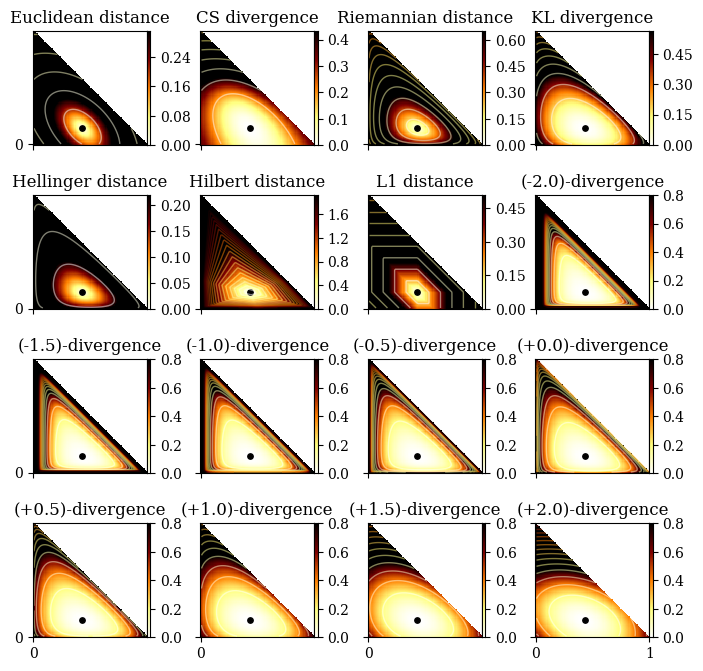
\includegraphics[width=\textwidth]{categories1}
\caption{Reference point (3/7,3/7,1/7)}
\end{subfigure}
\end{figure}

\begin{figure}\ContinuedFloat
\centering
\begin{subfigure}{\textwidth}
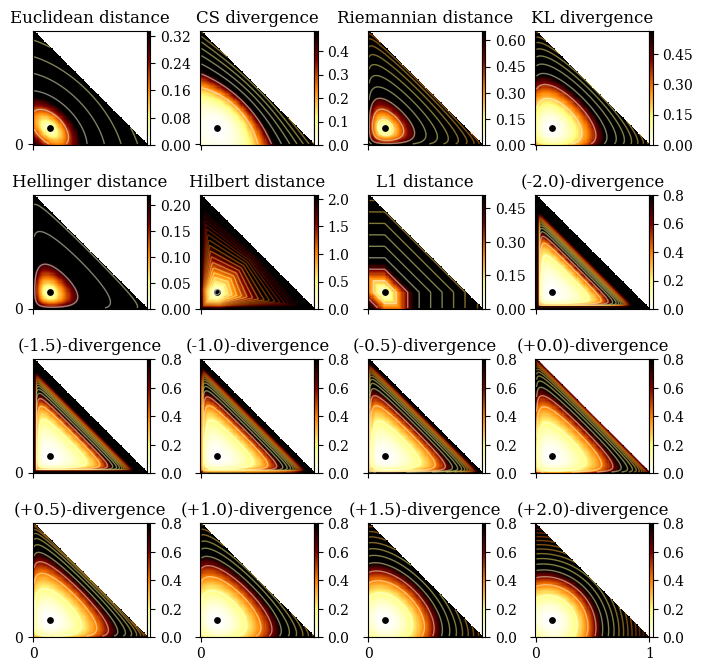
\includegraphics[width=\textwidth]{categories2}
\caption{Reference point (5/7,1/7,1/7)}
\end{subfigure}
\caption{A comparison of different distance measures on $\Delta^2$. The distance is measured from
$\forall{p}\in\Delta^2$ to a fixed reference point (the black dot). Lighter color means shorter
distance. Darker color means longer distance. The contours show equal distance curves with a precision step of $0.2$.\label{vis:distance}}
\end{figure}


%%%%%%%%%%%%%%%%%%%%%%%%%%%%%%%%%%%%%%%%%%%%%%%%%%%%%%%%%%%
\section{Center-based clustering}\label{sec:clustering}
%%%%%%%%%%%%%%%%%%%%%%%%%%%%%%%%%%%%%%%%%%%%%%%%%%%%%%%%%%%

We concentrate on comparing the efficiency of Hilbert simplex geometry for clustering multinomials.
We shall compare the experimental results of $k$-means++ and $k$-center multinomial clustering for
the three distances: Rao and Hilbert metric distances, and KL divergence.
We describe how to adapt those clustering algorithms to the Hilbert distance.

%%%%%%%%%%%%%
\subsection{$k$-means++ clustering}
%%%%%%%%%%%%%%%

The celebrated $k$-means clustering minimizes the sum of within-cluster variances,
where each cluster has a center representative element.
When dealing with $k=1$ cluster, the center (also called centroid or cluster prototype)
is the center of mass defined as the minimizer of
$$
E_D(\Lambda,c) = \frac{1}{n} \sum_{i=1}^n D(p_i:c),
$$
where $D(\cdot:\cdot)$ is a dissimilarity measure.
For an arbitrary $D$, the centroid $c$ may not be available in closed form. 
Nevertheless, using a generalization of the $k$-means++ initialization~\cite{kmeanspp-2007}
(picking randomly seeds), one can bypass the centroid computation,
and yet guarantee probabilistically a good clustering.

Let $C=\{c_1,\ldots, c_k\}$ denote the set of $k$ cluster centers.
Then the generalized $k$-means energy to be minimized is defined by:
$$
E_D(\Lambda,C) = \frac{1}{n}\sum_{i=1}^n \min_{j\in\{1,\ldots,k\}} D(p_i:c_j).
$$
By defining the distance $D(p,C)=\min_{j\in\{1,\ldots,k\}} D(p:c_j)$ of a point to a set,
we can rewrite the objective function as $E_D(\Lambda,C) = \frac{1}{n}\sum_{i=1}^n D(p_i,C)$.
Let $E_D^*(\Lambda,k)=\min_{C\ :\ |C|=k} E_D(\Lambda,C) $ denote the global minimum of
$E_D(\Lambda,C)$ wrt some given $\Lambda$ and $k$.

The $k$-means++ seeding proceeds for an arbitrary divergence $D$ as follows:
Pick uniformly at random at first seed $c_1$, and then iteratively choose the
$(k-1)$ remaining seeds according to the following probability distribution:
$$
\mathrm{Pr}(c_j=p_i) =
\frac{D(p_i,\{c_1,\ldots,c_{j-1}\})}
{\sum_{i=1}^n D(p_i,\{c_1,\ldots,c_{j-1}\})}
\quad(2\le{j}\le{k}).
$$
Since its inception (2007), this $k$-means++ seeding has been extensively studied~\cite{Bachem-2016}.
We state the general theorem established by~\cite{tJ-2013}:
\begin{theorem}[Generalized $k$-means++ performance, \cite{tJ-2013}]\label{thm:kmeansplus}
Let $\kappa_1$ and $\kappa_2$ be two constants such that $\kappa_1$ defines the
quasi-triangular inequality property:
$$
D(x:z) \leq \kappa_1 \left(D(x:y)+D(y:z)\right),\quad\forall{}x,y,z\in\Delta^d,
$$
and $\kappa_2$ handles the symmetry inequality:
$$
D(x:y)\leq \kappa_2 D(y:x),\quad\forall x,y\in\Delta^d.
$$
Then the generalized $k$-means++ seeding guarantees with high probability a configuration $C$ of cluster centers such that:
\begin{equation}\label{eq:kmperf}
E_D(\Lambda,C)\leq 2\kappa_1^2(1+\kappa_2)(2+\log k) E_D^*(\Lambda,k).
\end{equation}
\end{theorem}
The ratio $\frac{E_D(\Lambda,C)}{E_D^*(\Lambda,k)}$ is called the {\em competitive factor}.
The seminal result of ordinary $k$-means++ was shown~\cite{kmeanspp-2007} to be $8(2+\log{k})$-competitive.
When evaluating $\kappa_1$, one has to note that squared metric distances are not metric because they do not satisfy the triangular inequality.
For example, the squared Euclidean distance is not a metric but it satisfies the $2$-quasi triangular inequality with $\kappa_1=2$.

We state the following general performance theorem:
\begin{theorem}[$k$-means++ performance in a metric space]\label{theo:kmms}
In any metric space $(\calX,d)$,
the $k$-means++ wrt the squared metric distance $d^2$ is $16(2+\log k)$-competitive.
\end{theorem}
\begin{proof}
Since a metric distance is symmetric, it follows that $\kappa_2=1$.
Consider the quasi-triangular inequality property for the squared non-metric dissimilarity $d^2$:
\begin{eqnarray*}
d(p,q) \leq d(p,q)+d(q,r),\\
d^2(p,q) \leq (d(p,q)+d(q,r))^2,\\
d^2(p,q) \leq d^2(p,q)+d^2(q,r)+2d(p,q)d(q,r).
\end{eqnarray*}

Let us apply the inequality of arithmetic and geometric means\footnote{For positive values $a$ and $b$,
the arithmetic-geometric mean inequality states that $\sqrt{ab}\leq\frac{a+b}{2}$.}:
\begin{equation*}
\sqrt{d^2(p,q)d^2(q,r)} \leq \frac{d^2(p,q)+d^2(q,r)}{2}.
\end{equation*}

Thus we have
\begin{equation*}
d^2(p,q) \leq d^2(p,q)+d^2(q,r)+2d(p,q)d(q,r)\leq 2(d^2(p,q)+d^2(q,r)).
\end{equation*}
That is, the squared metric distance satisfies the $2$-approximate triangle inequality,
and $\kappa_1=2$. The result is straightforward from Theorem~\ref{thm:kmeansplus}.
\end{proof}

\begin{theorem}[$k$-means++ performance in a normed space]\label{theo:kmns}
In any normed space $(\calX,\Vert\cdot\Vert)$,
the $k$-means++ with $D(x:y)=\Vert{x-y}\Vert^2$ is $16(2+\log k)$-competitive.
\end{theorem}
\begin{proof}
%In an inner product space $(\calX,\inner{\cdot}{\cdot})$, we can define the norm $\|x\|=\sqrt{\inner{x}{x}}$ and induced distance $D(x,y)=\|x-y\|$.
%Furthermore, the parallelogram law holds in an inner product space: 
%$$
%2\|x\|^2 + 2\|y\|^2=\|x+y\|^2+\|x-y\|^2.
%$$
%It follows that 
%$$
%2\Vert{}x'-y'\Vert^2 + 2\Vert{}y'-z'\Vert^2
%= \Vert{}x'-z'\Vert^2 + \Vert{}x'-2y'+z'\Vert^2 
%\ge \Vert{}x'-z'\Vert^2.
%$$
%We get the $2$-quasi triangular inequality
%$$
%\|x'-z'\|^2 \leq 2\left( \|x'-y'\|^2\ + \|y'-z'\|^2 \right).
%$$
In any normed space $(\calX,\Vert\cdot\Vert)$, 
we have both $\Vert{x-y}\Vert=\Vert{y-x}\Vert$
and the triangle inequality:
$$
\Vert{}x-z\Vert\le\Vert{x-y}\Vert+\Vert{y-z}\Vert.
$$
The proof is very similar to the proof of Theorem~\ref{theo:kmms} and is omitted.

%Squaring this inequality, we get
%$$
%\Vert{}x-z\Vert^2  \le (\Vert{x-y}\Vert+\Vert{y-z}\Vert)^2=\Vert{x-y}\Vert^2 + \Vert{y-z}\Vert^2 + 2\Vert{x-y}\Vert\Vert{y-z}\Vert
%$$

%Using the arithmetic-geometric inequality, we have 
%$$
%\Vert{x-y}\Vert \Vert{y-z}\Vert \leq \frac{\Vert{x-y}^2 + \Vert{y-z}^2}{2}
%$$

%Therefore it comes that
%$$
%\Vert{}x-z\Vert^2
%\le(\Vert{x-y}\Vert+\Vert{y-z}\Vert)^2
%\le2(\Vert{x-y}\Vert^2+\Vert{y-z}\Vert^2).
%$$

%Therefore $\Vert\cdot\Vert^2$ satisfies the $2$-quasi triangular inequality
%($\kappa_1=2$).
%Furthermore, we have $\Vert{x-y}\Vert^2=\Vert{y-x}\Vert^2$ ($\kappa_2=1$).
%Plugging $\kappa_1=2$ and $\kappa_2=1$ into Eq.~\ref{eq:kmperf},
%we get the $16(2+\log k)$-competitive factor.
\end{proof}

Since any inner product space $(\calX,\inner{\cdot}{\cdot})$ has an induced norm 
$\Vert{x}\Vert=\sqrt{\inner{x}{x}}$, we have the following corollary.
\begin{corollary}
In any inner product space $(\calX,\inner{\cdot}{\cdot})$, 
the $k$-means++ with $D(x:y)=\inner{x-y}{x-y}$ is $16(2+\log k)$-competitive.
\end{corollary}

We need to report a bound for the squared Hilbert symmetric distance ($\kappa_2=1$).
In~\cite{BH-2014} (Theorem 3.3), it was shown that Hilbert geometry of a bounded convex domain $\calC$ is isometric to a normed vector space iff
$\calC$ is an open simplex:  $(\Delta^d,\rho_\HG)\simeq (V^d,\Vert\cdot\Vert_\NH)$, where $\Vert\cdot\Vert_\NH$ is the corresponding norm.
Therefore $\kappa_1=2$. We write ``$\NH$'' for short for this equivalent normed Hilbert geometry.
Appendix~\ref{sec:isometry} recalls the construction due to~\cite{HilbertHarpe-1991},
and shows the squared Hilbert distance fails the triangle inequality
and it is not a distance induced by an inner product.

%However, in a {\em finite} dimensional vector space, all norms are ``equivalent,'' meaning that there exist two positive constants $\alpha$ and $\beta$ such that:
%\begin{equation}\label{eq:equivnorm}
%\alpha \|v\|_2 \leq \|v\|_H \leq \beta \|v\|_2.
%\end{equation}
%Figure~\ref{fig:alphabeta} shows an empirical range of the ratio 
%$\frac{\Vert{v}\Vert_{\mathrm{H}}}{\Vert{v}\Vert_l}$ for $l=1,\cdots,4$.
%The ratio $\alpha$ and $\beta$ depend on the dimension of the simplex $\Delta^d$.
%For example, when $d=10$, one can observe that empirically $\alpha\approx0.7$, $\beta\approx1.4$.

%\begin{figure}[t]
%\centering\includegraphics[width=\textwidth]{alphabeta}
%\caption{The ratio $\frac{\Vert{v}\Vert_{\mathrm{H}}}{\Vert{v}\Vert_l}$ on
%$10^4$ randomly drawn $v$ for $l=1,2,3,4$ and $d=1,\dots,10$.}\label{fig:alphabeta}
%\end{figure}

%We therefore get the following lemma:
%\begin{lemma}[Quasi-triangular inequality in Hilbert simplex geometry]
%In a Hilbert simplex geometry, $\kappa_1\leq 2\left(\frac{\beta}{\alpha}\right)^2$.
%\end{lemma}

%The constants $\alpha$ and $\beta$ depend on the dimension of the Hilbert simplex geometry.

%\begin{proof}
%From $\alpha \|v\|_2 \leq \|v\|_H \leq \beta \|v\|_2$, we get:
%$$
%\alpha^2 \|v_p-v_q\|^2_2 \leq \rho^2_\HG(p,q) = \|v_p-v_q\|^2_H \leq \beta^2 \|v_p-v_q\|^2_2,
%$$
%where $v_p$ and $v_q$ are the equivalent points in the normed space corresponding to point $p$ and $q$, respectively.
%Let $D_E(v_p,v_q)=\|v_p-v_q\|$ denote the Euclidean distance.
%Since $\rho^2_\HG(p,q)\leq  \beta^2 D_E^2(v_p,v_q)$ and that $D_E^2$  satisfies the $2$-quasi-triangular inequality, we get:
%$$
%\rho^2_\HG(p,q)\leq  2\beta^2 (D_E^2(v_p,v_r) + D_E^2(v_r,v_q)),\quad\forall v_p,v_q,v_r\in V^d.
%$$
%But $D_E(v_x,v_y)^2 \leq \frac{1}{\alpha^2} \rho^2_\HG(x,y)$.
%It follows that:
%$$
%\rho^2_\HG(p,q)\leq  2\frac{\beta^2}{\alpha^2}(\rho^2_\HG(p,r) + \rho^2_\HG(r,q)).
%$$
%Therefore the squared Hilbert distance in a simplex satisfies the $\kappa_1$-triangular inequality for $\kappa_1=2\left(\frac{\beta}{\alpha}\right)^2$.
%\end{proof}

As an empirical study, we randomly generate $n=10^6$ tuples $(x, y, z)$ 
based on the uniform distribution in $\Delta^d$. For each tuple $(x,y,z)$,
we evaluate the ratio
$$
\kappa_1 = \frac{D(x:z)}{D(x:y)+D(y:z)}.
$$
Figure~\ref{fig:kappa} shows the statistics for four different choices of
$D$: (1) $D(x:y)=\rho_{\mathrm{FHR}}^2(x,y)$;
(2) $D(x:y)=\frac{1}{2}\KL(x:y)+\frac{1}{2}\KL(y:x)$;
(3) $D(x:y)=\rho^2_{\mathrm{HG}}(x,y)$;
(4) $D(x:y)= \rho^2_{\mathrm{L1}}(x,y)$.
We find experimentally that $\kappa_1$ is upper bounded by 2 for
$\rho^2_{\mathrm{FHR}}$, $\rho^2_{\mathrm{HG}}$
and $\rho^2_{\mathrm{L1}}$,
while the average $\kappa_1$ value is smaller than 0.5.
For all the compared distances, $\kappa_2=1$.
Therefore $\rho_{\mathrm{FHR}}$
and $\rho_{\mathrm{HG}}$ have better $k$-means++ performance guarantee as compared 
to $\rho_{\mathrm{IG}}$.


We get by applying Theorem~\ref{theo:kmns}:
\begin{corollary}[$k$-means++ in  Hilbert simplex geometry]
The $k$-means++ seeding in a  Hilbert simplex geometry in fixed dimension is $16 (2+\log k)$-competitive.
\end{corollary}


Figure~\ref{fig:kmresults} displays the clustering results of $k$-means++ in Hilbert simplex geometry as
compared to the other geometries for $k\in\{3,5\}$.

\begin{figure}[t]
\centering
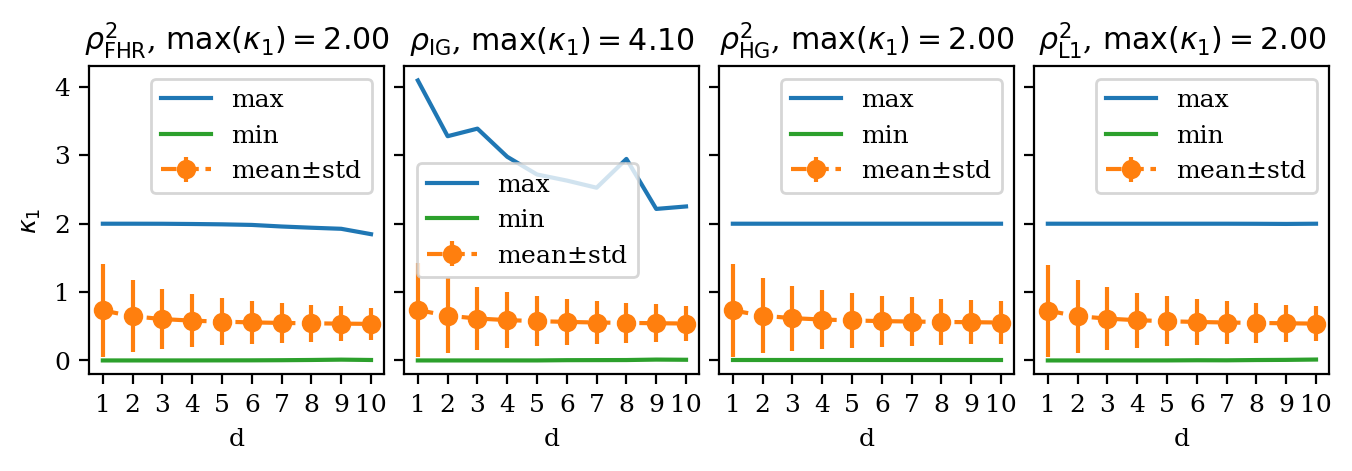
\includegraphics[width=\textwidth]{kappa}
\caption{The maximum, mean, standard deviation, and minimum
of $\kappa_1$ on $10^6$ randomly generated tuples $(x,y,z)$ in $\Delta^d$ for
$d=1,\dots,10$.}\label{fig:kappa}
\end{figure}

\begin{figure}[t]
\centering
\begin{subfigure}{\textwidth}
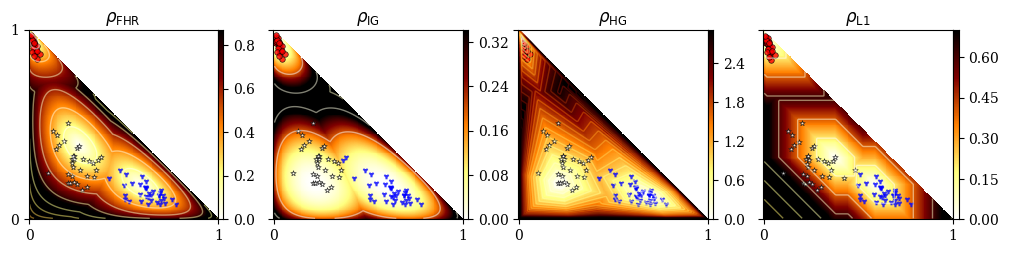
\includegraphics[width=\textwidth]{plusplus3}
\caption{$k=3$ clusters}
\end{subfigure}
\begin{subfigure}{\textwidth}
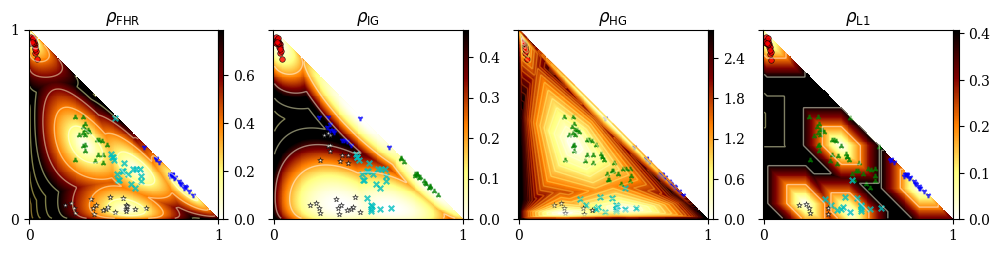
\includegraphics[width=\textwidth]{plusplus5}
\caption{$k=5$ clusters}
\end{subfigure}
\caption{$k$-Means++ clustering results on a toy dataset in the space of trinomials $\Delta^2$.
The color density maps indicate the distance from any point to its nearest cluster center.}\label{fig:kmresults}
\end{figure}

The KL divergence can be interpreted as a separable Bregman divergence~\cite{BregmanKmeans-2010}.
The Bregman $k$-means++ performance has been studied in~\cite{BregmanKmeans-2010,smoothedBregmankMeans-2013},
and a competitive factor of $O(\frac{1}{\mu})$ is reported using the notion of Bregman $\mu$-similarity (that is suited for data-sets on a compact domain).

In~\cite{sphericalkm-2015}, spherical $k$-means++ is studied wrt the distance $d_S(x,y)=1-\inner{x}{y}$ for any pair of points $x,y$ on the unit sphere. 
Since $\inner{x}{y}=\|x\|_2 \|y\|_2 \cos(\theta_{x,y})=\cos(\theta_{x,y})$, we have  $d_S(x,y)=1-\cos(\theta_{x,y})$, where $\theta_{x,y}$ 
denotes the angle between a pair of unit vectors $x$ and $y$. This distance is called the cosine distance since it amounts to one minus the cosine similarity.
Notice that the cosine distance is related to the squared Euclidean distance via the identity: $d_S(x,y)=\frac{1}{2}\|x-y\|^2$.
The cosine distance is different from the spherical distance that relies on the arccos function.

Since divergences may be asymmetric, one can further consider mixed divergence $M(p:q:r)=\lambda D(p:q)+(1-\lambda)D(q:r)$
for $\lambda\in[0,1]$, and extend the $k$-means++ seeding procedure and analysis~\cite{MixedClustering-2014}.

For a given data set, we can compute $\kappa_1$ or $\kappa_2$ by inspecting triples and pairs of points,
and get data-dependent competitive factor improving the bounds mentioned above.
 
%%%%%%%%%%%%
\subsection{$k$-Center clustering}
%%%%%%%%%%%%

Let $\Lambda$ be a finite point set.
The cost function for a $k$-center clustering with centers $C$ ($|C|=k$) is:
$$
f_D(\Lambda, C) = \max_{p_i\in\Lambda} \min_{c_j\in{}C} D(p_i\,:\,c_j).
$$
The farthest first traversal heuristic~\cite{kcenter-1985} has a guaranteed approximation factor of $2$ for any metric distance (see Algorithm~\ref{alg:kcenter}).

\begin{algorithm}[t]
\KwData{A set of points $p_1,\cdots,p_n\in\Delta^d$.  A distance measure $\rho$ on $\Delta^d$.
The maximum number $k$ of clusters. The maximum number $T$ of iterations.}
\KwResult{A clustering scheme assigning each $p_i$ a label $l_i\in\{1,\ldots,k\}$}
\Begin{
Randomly pick $k$ cluster centers $c_1,\ldots,c_k$ using
the kmeans\texttt{++} heuristic\;
\For{$t=1,\cdots,T$}{
%\tcc{Assign each sample to the nearest cluster}
\For{$i=1,\cdots,n$}{
  $l_i\leftarrow\argmin_{l=1}^k \rho(p_i, c_l)$\;
}
%\tcc{Recompute the cluster minimax centers}
\For{$l=1,\cdots,k$}{
  $c_l\leftarrow \argmin_c\max_{i:l_i=l} \rho(p_i,c)$\;
}
}
Output $\{l_i\}_{i=1}^n$\;
}
\caption{$k$-Center clustering}\label{alg:cluster}
\end{algorithm}

\begin{algorithm}
\KwData{A set $\Lambda$; a number $k$ of clusters; a metric distance $\rho$.}
\KwResult{A $2$-approximation of the $k$-center clustering}
\Begin{
$c_1\leftarrow\mathrm{ARandomPointOf}(\Lambda)$\;
$C\leftarrow\{c_1\}$\;
\For{$i=2,\cdots,{k}$}{
$c_i\leftarrow\arg\max_{p\in\Lambda} \rho(p,C)$\;
$C\leftarrow C\cup \{c_i\}$\;
}}
Output $C$\;
\caption{A $2$-approximation of the $k$-center clustering for any metric distance $\rho$.\label{alg:kcenter}}
\end{algorithm}

In order to use the $k$-center clustering algorithm described in Algorithm~\ref{alg:cluster},
we need to be able to compute the $1$-center (or minimax center) for the Hilbert simplex geometry,
that is the Minimum Enclosing Ball (MEB, also called the Smallest Enclosing Ball, SEB).

We may consider the SEB equivalently either in $\Delta^d$ or in the normed space $V^d$.
In both spaces, the shapes of the balls are convex.
Let $\Lambda=\{p_1,\ldots,p_n\}$ denote the point set in $\Delta^d$,
and $\calV=\{v_1,\ldots,v_n\}$ the equivalent point set in the normed vector space
(following the mapping explained in Appendix~\ref{sec:isometry}).
Then the SEBs $B_\HG(\Lambda)$ in $\Delta^d$ and $B_\NH(\calV)$ in $V^d$ have respectively radii $r^*_\HG$ and $r_\NH^*$ defined by:

\begin{eqnarray*}
r^*_\HG &=& \min_{c\in\Delta^d}  \max_{i\in\{1,\ldots, n\}} \rho_\HG(p_i,c),\\
r^*_\NH &=& \min_{v\in V^d}      \max_{i\in\{1,\ldots, n\}} \|v_i-v\|_\NH.
\end{eqnarray*}

%It follows from the inequalities of Eq.~\ref{eq:equivnorm} that: $$ \alpha r_E^* \leq r_H \leq \beta r_E^*, $$
%where $r_E^*$ is the radius of the SEB with respect to the Euclidean distance of the points $v_1\ldots,v_n$.

The SEB in the normed vector space $(V^d,\|\cdot\|_\NH)$ amounts to find the minimum covering norm polytope  of a finite point set.
This problem has been well-studied in computational geometry~\cite{Saha-2011,Brandenberg-2013,EnclosingPolytope-2004}.
By considering the equivalent Hilbert norm polytope with $d(d+1)$ facets, we state the result of~\cite{Saha-2011}:

\begin{theorem}[SEB in Hilbert polytope normed space,~\cite{Saha-2011}]
A $(1+\epsilon)$-approximation of the SEB in $V^d$ can be computed in $O(d^3\frac{n}{\epsilon})$ time.
\end{theorem}

We shall now report two algorithms for computing the SEBs: One exact algorithm in $V^d$ that does not scale well in high dimensions,
and one approximation in $\Delta^d$ that works well for large dimensions.

%%%%%%
\subsubsection{Exact smallest enclosing ball in a Hilbert simplex geometry\label{sec:SEBHSG}} 
%%%%%%

Given a finite point set $\{p_1,\ldots, p_n\}\in\Delta^d$, the SEB in Hilbert simplex geometry
is centered at
\begin{equation*}
c^*=\argmin_{c\in \Delta^d} \max_{i\in\{1,\ldots,n\}} \rho_\HG(c,x_i),
\end{equation*}
with radius
\begin{equation*}
r^*=\min_{c\in \Delta^d} \max_{i\in\{1,\ldots,n\}} \rho_\HG(c,x_i).
\end{equation*}

An equivalent problem is to find the SEB in the isometric normed vector space $V^d$
via the mapping reported in Appendix~\ref{sec:isometry}.
Each simplex point $p_i$ corresponds to a point $v_i$ in the $V^d$.

%First, recenter the $n$ vector points $v_1,\ldots, v_n$ so that $\frac{1}{n}\sum_i v_i=0$.
%Then let us place the norm unit ball $B_V=\{v\in V^d \st \|v\|_H\leq 1\}$ at the origin, and let us find the smallest {\em homothetic factor} $r^*\geq 0$ 
%such that $\forall i, v_i\in r^*\times B_V$.
%Since the norm is a polytope norm (the intersection of $d(d+1)$ halfspaces passing through the facets and containing the origin),
%finding the SEB in the vector space amounts to find the minimum radius $r^*\ geq 0$ such that:
%\begin{equation}
%\forall i\not=j, \forall l\in\{1,\ldots, n\},   (v^i_l-v^j_l) \leq r^*,   (v^j_l-v^i_l) \geq -r^*
%\end{equation}
%
%This optimization problem is a Linear Program (LP) in dimension $d+1$ with $d(d+1)n$ constraints.
%Geometrically speaking, each facet of the Hilbert polytope norm $\|\cdot\|_H$  is supported by a hyperplane yielding a linear constraint.
%When the dimension is fixed, solving a LP can be done linearly in the number of constraints.
%Once the optimal enclosing ball in the vector space is found, we map it back to get the corresponding SEB in the Hilbert geometry.
%Therefore the Hilbert SEB can be computed exactly in linear time in fixed dimension.
%
%\begin{theorem}[SEB in Hilbert simplex]
%The Smallest Enclosing Ball in Hilbert simplex geometry of fixed dimension can be computed exactly in linear time using linear programming.
%\end{theorem}


Figure~\ref{fig:SEB} displays some examples of the exact smallest enclosing balls in the Hilbert simplex geometry and in the corresponding normed vector space.

\begin{figure}[t]
\centering
\begin{subfigure}[m]{.48\textwidth}
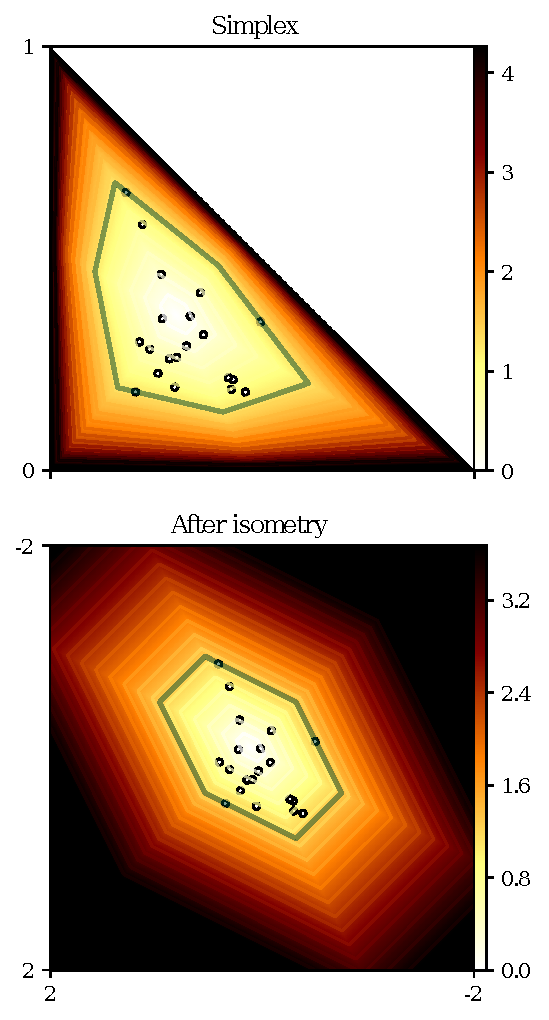
\includegraphics[width=.5\textwidth]{harpe2017.pdf}%
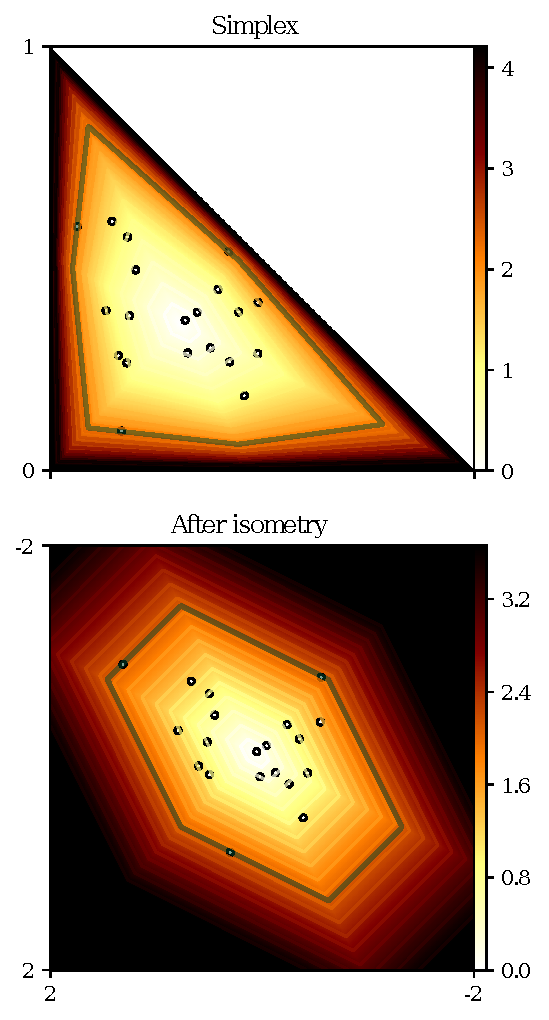
\includegraphics[width=.5\textwidth]{harpe2026.pdf}
\caption{$3$ points on the border}
\end{subfigure}
\begin{subfigure}[m]{.48\textwidth}
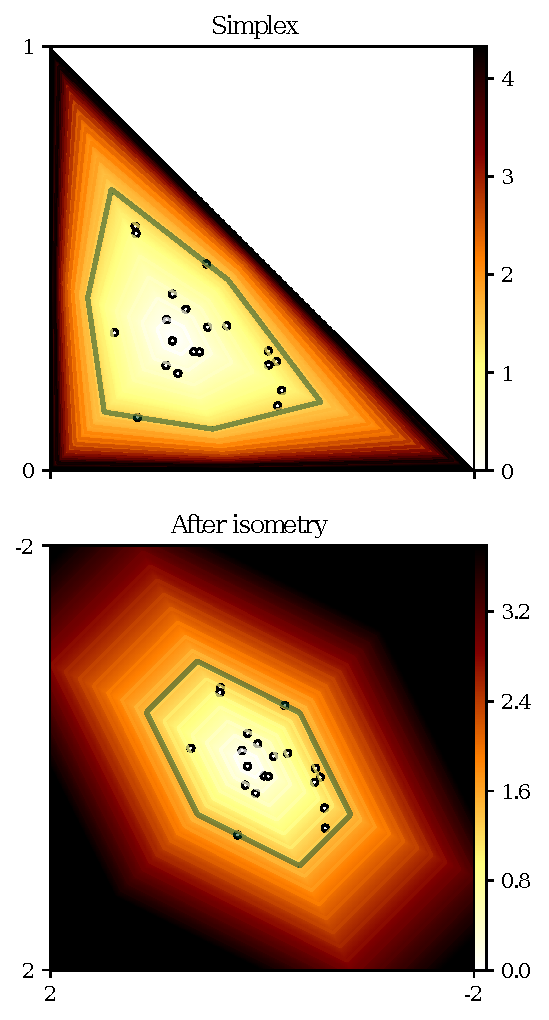
\includegraphics[width=.5\textwidth]{harpe2020.pdf}%
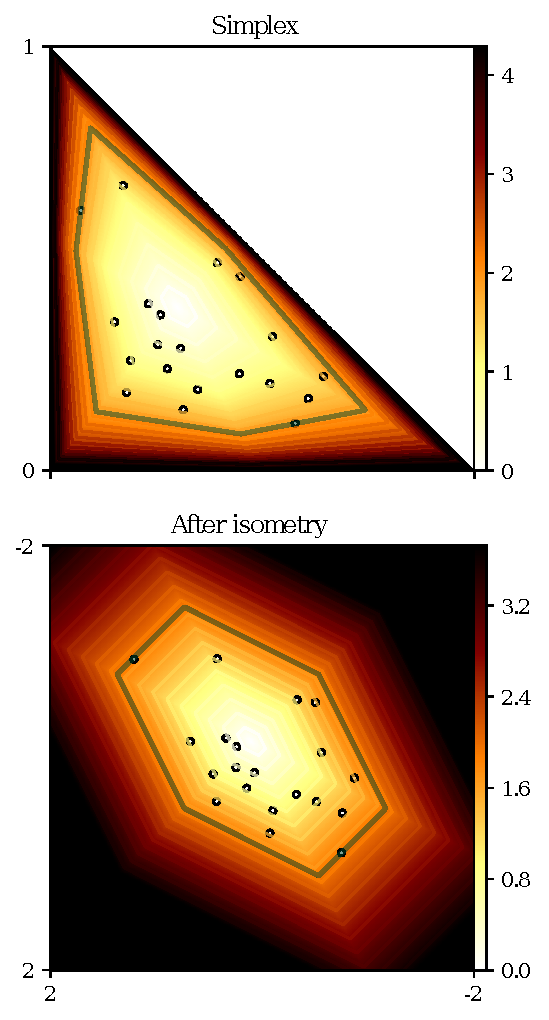
\includegraphics[width=.5\textwidth]{harpe2028.pdf}
\caption{$2$ points on the border}
\end{subfigure}
\caption{Computing the SEB in Hilbert simplex geometry
amounts to compute the SEB in the corresponding normed
vector space.\label{fig:SEB}}
\end{figure}

To compute the SEB, one may also consider the generic LP-type randomized algorithm~\cite{SEBB-2008}.
We notice that an enclosing ball for a point set in general has
a number $k$ of points on the border of the ball, with $2\leq k\leq \frac{d(d+1)}{2}$.
Let $D=\frac{d(d+1)}{2}$ denote the varying size of the combinatorial basis,
then we can apply the LP-type framework (we check the axioms of locality and monotonicity,~\cite{LPtype-1992})
to solve efficiently the SEBs. 

\begin{theorem}[Smallest Enclosing Hilbert Ball is LP-type,~\cite{Welzl-1991,LPtype-1992}]
The smallest enclosing Hilbert ball amounts to find the smallest enclosing ball in a vector space
wrt a polytope norm that can be solved using a LP-type randomized algorithm.
\end{theorem}

The Enclosing Ball Decision Problem~(EBDP, \cite{BallML-2009}) asks for a given value $r$, whether $r\geq r^*$ or not.
The decision problem amounts to find whether a set $\{rB_V+v_i\}$ of translates can be stabbed by a point~\cite{BallML-2009}:
That is, whether $\cap_{i=1}^n (rB_V+v_i)$ is empty or not. Since these translates are polytopes with $d(d+1)$ facets,
this can be solved in linear time using {\em Linear Programming}.

\begin{theorem}[Enclosing Hilbert Ball Decision Problem]
The decision problem to test whether $r\geq r^*$ or not can be solved by Linear Programming.
\end{theorem}

This yields a simple scheme to approximate the optimal value $r^*$: 
Let $r_0=\max_{i\in\{2,\ldots,n\}} \|v_i-v_1\|_\NH$. Then $r^*\in[\frac{r_0}{2},r_0]=[a_0,b_0]$.
At stage $i$, perform a dichotomic search on $[a_i,b_i]$ by answering the decision problem for
$r_{i+1}=\frac{a_i+b_i}{2}$, and update the radius range accordingly~\cite{BallML-2009}.
 
However, the LP-type randomized algorithm or the decision problem-based algorithm do not scale well in high dimensions.
Next, we introduce a simple approximation algorithm that relies on the fact that the line segment $[pq]$ is a geodesic in Hilbert simplex geometry.
(Geodesics are not unique. See Figure~2 of~\cite{HilbertHarpe-1991}.)

\subsubsection{Geodesic bisection approximation heuristic\label{sec:BCHSG}} 

In Riemannian geometry, the $1$-center can be arbitrarily finely approximated by
a simple geodesic bisection algorithm~\cite{bc-2003,miniball-2013}.
This algorithm can be extended to HG straightforwardly as detailed in Algorithm~\ref{alg:center}.

\begin{algorithm}
\KwData{A set of points $p_1,\cdots,p_n\in\Delta^d$. The maximum number $T$ of iterations.}
\KwResult{$c\approx\argmin_c\max_i\rho_{\mathrm{HG}}(p_i,c)$}
\Begin{
%$c_0\leftarrow\frac{1}{n}\sum_{i=1}^n p_i$\;
$c_0\leftarrow\mathrm{ARandomPointOf}(\{p_1,\cdots,p_n\})$\;
\For{$t=1,\cdots,T$}{
$p\leftarrow\argmax_{p_i}\rho_{\mathrm{HG}}(p_i,c_{t-1})$\;
$c_t\leftarrow c_{t-1} \#_{1/(t+1)}^\rho p$\;
}
Output $c_{T}$\;
}
\caption{Geodesic walk for approximating the Hilbert minimax center, generalizing~\cite{bc-2003}}\label{alg:center}
\end{algorithm}

\begin{figure}[ht]
\centering
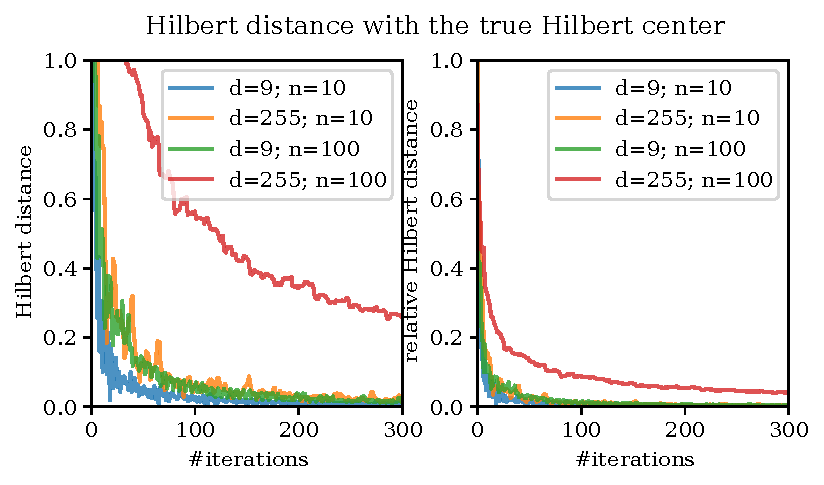
\includegraphics[width=\textwidth]{convergence}
\caption{Convergence rate of Alg.~(\ref{alg:center})
measured by the Hilbert distance between the current minimax center and the true center (left)
or their Hilbert distance divided by the Hilbert radius of the dataset (right).
The plot is based on $100$ random points in $\Delta^{9}$/$\Delta^{255}$.}\label{fig:convergence}
\end{figure}

\begin{figure}[htb]
\centering
\begin{subfigure}[m]{.7\textwidth}
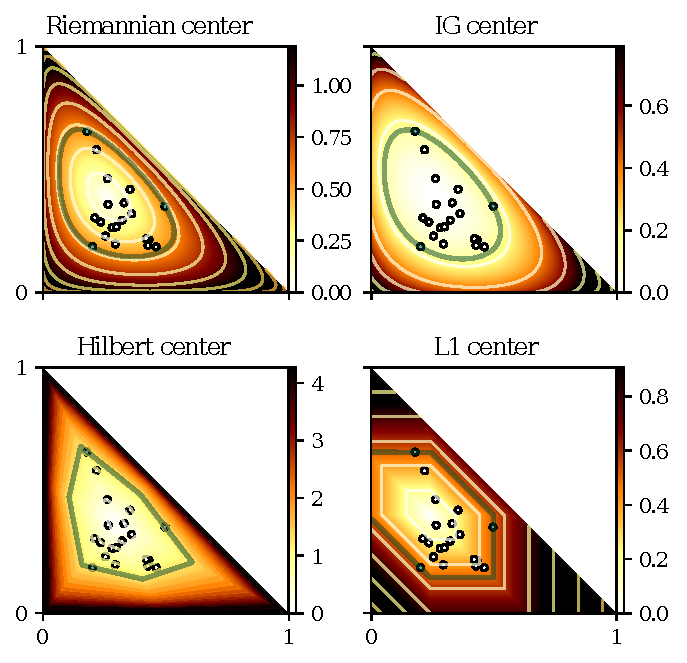
\includegraphics[width=\textwidth]{center1}%
\caption{Point Cloud 1}
\end{subfigure}
\begin{subfigure}[m]{.7\textwidth}
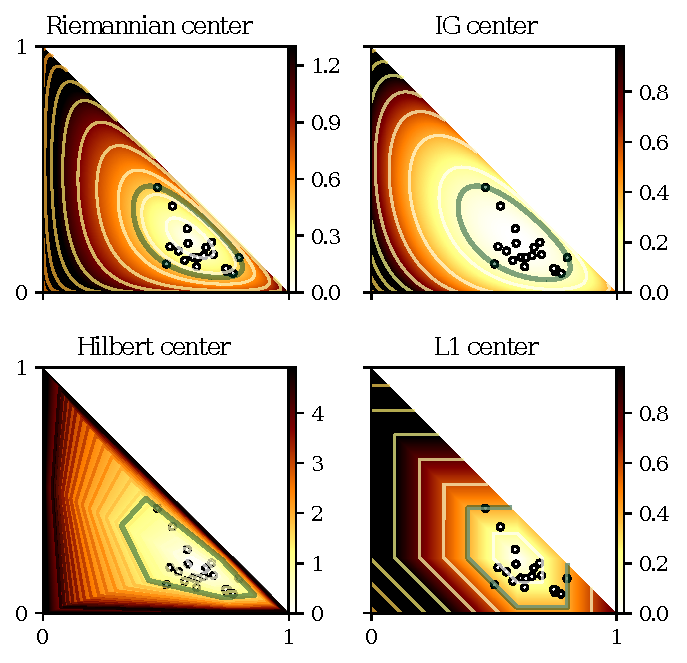
\includegraphics[width=\textwidth]{center2}%
\caption{Point Cloud 2}
\end{subfigure}
\end{figure}

\begin{figure}[!htb]\ContinuedFloat
\centering
\begin{subfigure}[m]{.7\textwidth}
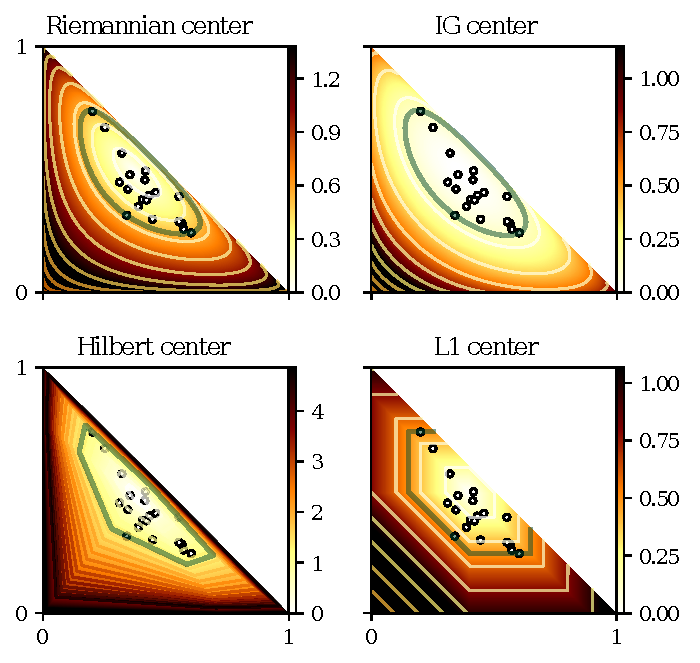
\includegraphics[width=\textwidth]{center3}%
\caption{Point Cloud 3}
\end{subfigure}
\caption{The Riemannian/IG/Hilbert/$L_1$  minimax centers of three point clouds
in $\Delta^2$ based on Alg.~(\ref{alg:center}).
The color maps show the distance from $\forall{p}\in\Delta^2$ to the corresponding center.}
\label{fig:center}
\end{figure}

The algorithm first picks up a point $c_0$ at random from $\Lambda$ as the initial center,
then computes the farthest point $p$ (with respect to the distance $\rho$),
and then walk on the geodesic from $c_0$ to $p$ by a certain amount to define $c_1$, etc. 
For an arbitrary distance $\rho$, we define the operator $\#^\rho_\alpha$ as follows:
$$
p \#^\rho_\alpha q = v=\gamma(p,q,\alpha), \quad \rho(p:v)=\alpha \rho(p:q),
$$
where $\gamma(p,q,\alpha)$ is the geodesic passing through $p$ and $q$, and parameterized by $\alpha$ ($0\le\alpha\le1$).
When the equations of the geodesics are explicitly known, we can either get a closed form solution for $\#^\rho_\alpha$
or perform a bisection search to find $v'$ such that $\rho(p:v')\approx\alpha\rho(p:q)$.
See~\cite{ApproximatingHyperbolicBall-2015} for an extension and analysis in hyperbolic geometry.
See Fig.~(\ref{fig:convergence}) to get an intuitive idea on the {\em experimental} convergence rate of Algorithm~\ref{alg:center}.
See Fig.~(\ref{fig:center}) for visualizations of centers wrt different geometries.

Furthermore, this iterative algorithm implies a core-set~\cite{coreset-2008} (namely, the set of farthest points visited during the geodesic walks)
that is useful for clustering large data-sets~\cite{coreset-2017}.
See~\cite{Brandenberg-2013} for core-set results on containment problems
wrt a convex homothetic object (the equivalent Hilbert polytope norm in our case).

A simple algorithm dubbed {\sc MinCon} \cite{EnclosingPolytope-2004} 
can find an approximation of the Minimum Enclosing Polytope.
The algorithm induces a core-set of size $O(\frac{1}{\eps^2})$ although the theorem is challenged in~\cite{Brandenberg-2013}.

Thus by combining the $k$-center seeding \cite{kcenter-1985} with the Lloyd-like batched iterations, we get an efficient $k$-center clustering
algorithm for the FHR and Hilbert metric geometries.
When dealing with the Kullback-Leibler divergence, we use the fact that KL is a Bregman divergence, and
use the $1$-center algorithm~(\cite{BregmanMinimax-2005,BregmanBall-2006} for approximation in any dimension,
or \cite{SEBB-2008} which is exact but limited to small dimensions).

Since Hilbert simplex geometry is isomorphic to a normed vector space~\cite{BH-2014} with
a polytope norm with $d(d+1)$ facets, the Voronoi diagram in Hilbert geometry of $\Delta^d$ amounts to 
compute a Voronoi diagram wrt a polytope norm~\cite{MinisumHypersphere-2011,VoronoiNorm-2012,voronoi-2015}.

%%%%%%%%%%%%%
\section{Experiments}\label{sec:exp}
%%%%%%%%%%%%
We generate a dataset consisting of a set of clusters in a high dimensional statistical simplex $\Delta^d$.
Each cluster is generated independently as follows. We first pick a
random center $c=(\lambda_c^0,\ldots,\lambda_c^d)$ based on the uniform distribution on $\Delta^d$.
Then any random sample $p=(\lambda^0,\ldots,\lambda^d)$ associated with $c$ is independently generated by
$$
\lambda^i = \frac{\exp(\log\lambda_c^i + \sigma\epsilon^i)}{\sum_{i=0}^d \exp(\log\lambda_c^i + \sigma\epsilon^i) },
$$
where $\sigma>0$ is a noise level parameter, and each $\epsilon^i$ follows independently
a standard Gaussian distribution (generator 1) or the Student's $t$-distribution
with five degrees of freedom (generator 2).
Let $\sigma=0$, we get $\lambda^i=\lambda_c^i$. Therefore $p$ is randomly distributed around $c$.
We repeat generating random samples for each cluster center, and make sure
that different clusters have almost the same number of samples. Then we 
perform clustering based on the configurations
$n\in\{50,100\}$, $d\in\{9,255\}$, $\sigma\in\{0.5,0.9\}$,
$\rho\in\{\rho_{\mathrm{FHR}}, \rho_{\mathrm{IG}}, \rho_{\mathrm{HG}},
\rho_{\mathrm{EUC}}, \rho_{\mathrm{L1}}\}$.
For simplicity, the number of clusters $k$ is set to the ground truth.
For each
configuration, we repeat the clustering experiment based on 300 different random
datasets. The performance is measured by the normalized mutual information (NMI),
which is a scalar indicator in the range $[0,1]$ (the larger the better).

The results of $k$-means++ and $k$-centers are shown in Table~\ref{tbl:plusplus}
and Table~\ref{tbl:results}, respectively. The large variance of NMI is because
that each experiment is performed on random datasets wrt different random seeds.
Generally, the performance deteriorates as we increase the number of clusters,
increase the noise level or decrease the dimensionality,
which have the same effect to reduce the inter-cluster gap.

The key comparison is the three columns $\rho_{\mathrm{FHR}}$, $\rho_{\mathrm{HG}}$
and $\rho_{\mathrm{IG}}$, as they are based on exactly the same algorithm
with the only difference being the underlying geometry.
We see clearly that in general their clustering performance presents the order $\mathrm{HG}>\mathrm{FHR}>\mathrm{IG}$.
The performance of HG is superior to the other two geometries, especially when the noise level is large.
Intuitively, the Hilbert balls are more compact in size and
therefore can better capture the clustering structure (see Fig.~(\ref{fig:results})).

%In Table~\ref{tbl:results},
%the column $\rho_{\mathrm{IG}}$ ($k$-means) is the k-means clustering
%based on $\rho_{\mathrm{IG}}$. It shows better performance than $\rho_{\mathrm{IG}}$
%because $k$-means is more robust than $k$-center to noise.
%Ideally we should compare $k$-means based on $\mathrm{FHR}$, $\mathrm{IG}$ and $\mathrm{HG}$.
%However the centroid computation of $\mathrm{FHR}$ and $\mathrm{HG}$ are not 
%developed yet. This is left to future work.

The column $\rho_{\mathrm{EUC}}$ is based on the Euclidean enclosing
ball. It shows the worst scores because the intrinsic geometry of the
probability simplex is far from the Euclidean geometry.

%Notice that at high dimensions when $\rho_{\mathrm{IG}}$ ($k$-means) shows favorable 
%performance, $\rho_{\mathrm{HG}}$ ($k$-centers) is still comparable.

\begin{table*}
\centering
\caption{$k$-means++ clustering accuracy in NMI on randomly generated datasets
based on different geometries. The table shows
the mean and standard deviation after 300 independent runs for each configuration.
$\rho$ is the distance measure. $n$ is the sample size.
$d$ is the dimensionality of $\Delta^d$. $\sigma$ is noise level.}\label{tbl:plusplus}
\begin{tabular}{c|c|c|c|ccccc}
\toprule[1.5pt]
$k$ & $n$ & $d$ & $\sigma$ & $\rho_{\mathrm{FHR}}$ & $\rho_{\mathrm{IG}}$ & $\rho_{\mathrm{HG}}$ & $\rho_{\mathrm{EUC}}$ & $\rho_{L1}$\\\hline
\multirow{12}{*}{3}
&\multirow{6}{*}{50} &\multirow{3}{*}{$9$}
  & $0.5$ & $0.76\pm0.22$ & $0.76\pm0.24$ & $\bm{0.81\pm0.22}$ & $0.64\pm0.23$ & $0.70\pm0.22$ \\
&&& $0.9$ & $0.44\pm0.20$ & $0.44\pm0.20$ & $\bm{0.57\pm0.22}$ & $0.31\pm0.17$ & $0.38\pm0.18$ \\\cline{3-9}
&&\multirow{3}{*}{$255$}
  & $0.5$ & $0.80\pm0.24$ & $0.81\pm0.24$ & $\bm{0.88\pm0.21}$ & $0.74\pm0.25$ & $0.79\pm0.24$ \\
&&& $0.9$ & $0.65\pm0.27$ & $0.66\pm0.28$ & $\bm{0.72\pm0.27}$ & $0.46\pm0.24$ & $0.63\pm0.27$ \\\cline{2-9}
&\multirow{6}{*}{100}
&\multirow{3}{*}{$9$}
 &  $0.5$ & $0.76\pm0.22$ & $0.76\pm0.21$ & $\bm{0.82\pm0.22}$ & $0.60\pm0.21$ & $0.69\pm0.23$ \\
&&& $0.9$ & $0.42\pm0.19$ & $0.41\pm0.18$ & $\bm{0.54\pm0.22}$ & $0.27\pm0.14$ & $0.34\pm0.16$ \\\cline{3-9}
&& \multirow{3}{*}{$255$}
  & $0.5$ & $0.82\pm0.23$ & $0.82\pm0.24$ & $\bm{0.89\pm0.20}$ & $0.74\pm0.24$ & $0.80\pm0.25$ \\
&&& $0.9$ & $0.66\pm0.26$ & $0.66\pm0.28$ & $\bm{0.72\pm0.26}$ & $0.45\pm0.25$ & $0.64\pm0.27$ \\\cline{1-9}
\multirow{12}{*}{5}
& \multirow{6}{*}{50}
& \multirow{3}{*}{9}
  & $0.5$ & $0.75\pm0.14$ & $0.74\pm0.15$ & $\bm{0.81\pm0.13}$ & $0.61\pm0.13$ & $0.68\pm0.13$ \\
&&& $0.9$ & $0.44\pm0.13$ & $0.42\pm0.13$ & $\bm{0.55\pm0.15}$ & $0.31\pm0.11$ & $0.36\pm0.12$ \\\cline{3-9}
&& \multirow{3}{*}{$255$}
  & $0.5$ & $0.83\pm0.15$ & $0.83\pm0.15$ & $\bm{0.88\pm0.14}$ & $0.77\pm0.16$ & $0.82\pm0.15$ \\
&&& $0.9$ & $0.71\pm0.17$ & $0.70\pm0.19$ & $\bm{0.75\pm0.17}$ & $0.50\pm0.17$ & $0.68\pm0.18$ \\\cline{2-9}
&\multirow{6}{*}{100}
& \multirow{3}{*}{$9$}
  & $0.5$ & $0.74\pm0.13$ & $0.74\pm0.14$ & $\bm{0.80\pm0.14}$ & $0.60\pm0.13$ & $0.67\pm0.13$ \\
&&& $0.9$ & $0.42\pm0.11$ & $0.40\pm0.12$ & $\bm{0.55\pm0.15}$ & $0.29\pm0.09$ & $0.35\pm0.11$ \\\cline{3-9}
&& \multirow{3}{*}{$255$}
  & $0.5$ & $0.83\pm0.14$ & $0.83\pm0.15$ & $\bm{0.88\pm0.13}$ & $0.77\pm0.15$ & $0.81\pm0.15$ \\
&&& $0.9$ & $0.69\pm0.18$ & $0.69\pm0.18$ & $\bm{0.73\pm0.17}$ & $0.48\pm0.17$ & $0.67\pm0.18$ \\
\bottomrule[1.5pt]
\end{tabular}
\\(a) generator 1\\\vspace{1em}
\begin{tabular}{c|c|c|c|ccccc}
\toprule[1.5pt]
$k$ & $n$ & $d$ & $\sigma$ & $\rho_{\mathrm{FHR}}$ & $\rho_{\mathrm{IG}}$ & $\rho_{\mathrm{HG}}$ & $\rho_{\mathrm{EUC}}$ & $\rho_{L1}$\\\hline
\multirow{12}{*}{3}
&\multirow{6}{*}{50} &\multirow{3}{*}{$9$}
  & $0.5$ & $0.62\pm0.22$ & $0.60\pm0.22$ & $\bm{0.71\pm0.23}$ & $0.45\pm0.20$ & $0.54\pm0.22$ \\
&&& $0.9$ & $0.29\pm0.17$ & $0.27\pm0.16$ & $\bm{0.39\pm0.19}$ & $0.17\pm0.13$ & $0.25\pm0.15$ \\\cline{3-9}
&&\multirow{3}{*}{$255$}
  & $0.5$ & $0.70\pm0.25$ & $0.69\pm0.26$ & $\bm{0.74\pm0.25}$ & $0.37\pm0.29$ & $0.70\pm0.26$ \\
&&& $0.9$ & $\bm{0.42\pm0.25}$ & $0.35\pm0.20$ & $0.40\pm0.19$ & $0.03\pm0.08$ & $\bm{0.44\pm0.26}$ \\\cline{2-9}
&\multirow{6}{*}{100}
&\multirow{3}{*}{$9$}
 &  $0.5$ & $0.63\pm0.22$ & $0.61\pm0.22$ & $\bm{0.71\pm0.22}$ & $0.46\pm0.19$ & $0.56\pm0.20$ \\
&&& $0.9$ & $0.29\pm0.15$ & $0.26\pm0.14$ & $\bm{0.38\pm0.20}$ & $0.18\pm0.12$ & $0.24\pm0.14$ \\\cline{3-9}
&& \multirow{3}{*}{$255$}
  & $0.5$ & $0.71\pm0.26$ & $0.69\pm0.27$ & $\bm{0.75\pm0.25}$ & $0.31\pm0.28$ & $0.70\pm0.27$ \\
&&& $0.9$ & $0.41\pm0.26$ & $0.33\pm0.20$ & $0.38\pm0.18$ & $0.02\pm0.06$ & $\bm{0.43\pm0.26}$ \\\cline{1-9}
\multirow{12}{*}{5}
& \multirow{6}{*}{50}
& \multirow{3}{*}{9}
  & $0.5$ & $0.64\pm0.15$ & $0.61\pm0.14$ & $\bm{0.70\pm0.14}$ & $0.48\pm0.14$ & $0.57\pm0.15$ \\
&&& $0.9$ & $0.31\pm0.12$ & $0.29\pm0.12$ & $\bm{0.41\pm0.15}$ & $0.20\pm0.09$ & $0.26\pm0.10$ \\\cline{3-9}
&& \multirow{3}{*}{$255$}
  & $0.5$ & $0.74\pm0.17$ & $0.72\pm0.17$ & $\bm{0.77\pm0.16}$ & $0.41\pm0.20$ & $0.74\pm0.17$ \\
&&& $0.9$ & $0.44\pm0.17$ & $0.37\pm0.16$ & $0.44\pm0.15$ & $0.04\pm0.06$ & $\bm{0.47\pm0.17}$ \\\cline{2-9}
&\multirow{6}{*}{100}
& \multirow{3}{*}{$9$}
  & $0.5$ & $0.62\pm0.14$ & $0.61\pm0.14$ & $\bm{0.71\pm0.14}$ & $0.46\pm0.13$ & $0.54\pm0.14$ \\
&&& $0.9$ & $0.30\pm0.10$ & $0.27\pm0.11$ & $\bm{0.40\pm0.13}$ & $0.19\pm0.08$ & $0.25\pm0.09$ \\\cline{3-9}
&& \multirow{3}{*}{$255$}
  & $0.5$ & $0.73\pm0.18$ & $0.70\pm0.18$ & $\bm{0.75\pm0.16}$ & $0.37\pm0.20$ & $0.73\pm0.17$ \\
&&& $0.9$ & $0.43\pm0.16$ & $0.35\pm0.14$ & $0.41\pm0.12$ & $0.03\pm0.06$ & $\bm{0.46\pm0.18}$ \\
\bottomrule[1.5pt]
\end{tabular}
\\(b) generator 2
\end{table*}

\begin{table*}
\centering\caption{$k$-center clustering accuracy in NMI on randomly generated datasets
based on different geometries. The table shows
the mean and standard deviation after 300 independent runs for each configuration.
$\rho$ is the distance measure. $n$ is the sample size.
$d$ is the dimensionality of the statistical simplex.
$\sigma$ is noise level.}\label{tbl:results}
\begin{tabular}{c|c|c|c|ccccc}
\toprule[1.5pt]
$k$ & $n$ & $d$ & $\sigma$ & $\rho_{\mathrm{FHR}}$ & $\rho_{\mathrm{IG}}$ & $\rho_{\mathrm{HG}}$ & $\rho_{\mathrm{EUC}}$ & $\rho_{L1}$\\\hline
\multirow{12}{*}{3}
&\multirow{6}{*}{50} &\multirow{3}{*}{$9$}
  & $0.5$ & $0.87\pm0.19$ & $0.85\pm0.19$ & $\bm{0.92\pm0.16}$ & $0.72\pm0.22$ & $0.80\pm0.20$ \\
&&& $0.9$ & $0.54\pm0.21$ & $0.51\pm0.21$ & $\bm{0.70\pm0.23}$ & $0.36\pm0.17$ & $0.44\pm0.19$ \\\cline{3-9}
&&\multirow{3}{*}{$255$}
  & $0.5$ & $0.93\pm0.16$ & $0.92\pm0.18$ & $\bm{0.95\pm0.14}$ & $0.89\pm0.18$ & $0.90\pm0.19$ \\
&&& $0.9$ & $0.76\pm0.24$ & $0.72\pm0.26$ & $\bm{0.82\pm0.24}$ & $0.50\pm0.28$ & $0.76\pm0.25$ \\\cline{2-9}
&\multirow{6}{*}{100}
&\multirow{3}{*}{$9$}
 &  $0.5$ & $0.88\pm0.17$ & $0.86\pm0.18$ & $\bm{0.93\pm0.14}$ & $0.70\pm0.20$ & $0.80\pm0.20$ \\
&&& $0.9$ & $0.53\pm0.20$ & $0.49\pm0.19$ & $\bm{0.70\pm0.22}$ & $0.33\pm0.14$ & $0.41\pm0.18$ \\\cline{3-9}
&& \multirow{3}{*}{$255$}
  & $0.5$ & $0.93\pm0.16$ & $0.92\pm0.17$ & $\bm{0.95\pm0.13}$ & $0.88\pm0.19$ & $0.93\pm0.16$ \\
&&& $0.9$ & $0.81\pm0.22$ & $0.75\pm0.24$ & $\bm{0.83\pm0.22}$ & $0.47\pm0.28$ & $0.79\pm0.22$ \\\cline{1-9}
\multirow{12}{*}{5}
& \multirow{6}{*}{50}
& \multirow{3}{*}{9}
  & $0.5$ & $0.82\pm0.13$ & $0.81\pm0.13$ & $\bm{0.89\pm0.12}$ & $0.67\pm0.13$ & $0.75\pm0.13$ \\
&&& $0.9$ & $0.50\pm0.13$ & $0.47\pm0.13$ & $\bm{0.66\pm0.15}$ & $0.34\pm0.11$ & $0.40\pm0.12$ \\\cline{3-9}
&& \multirow{3}{*}{$255$}
  & $0.5$ & $\bm{0.92\pm0.11}$ & $\bm{0.91\pm0.12}$ & $\bm{0.93\pm0.11}$ & $0.87\pm0.13$ & $\bm{0.92\pm0.12}$ \\
&&& $0.9$ & $0.77\pm0.15$ & $0.71\pm0.17$ & $\bm{0.85\pm0.17}$ & $0.54\pm0.19$ & $0.74\pm0.16$ \\\cline{2-9}
&\multirow{6}{*}{100}
& \multirow{3}{*}{$9$}
  & $0.5$ & $0.83\pm0.12$ & $0.81\pm0.13$ & $\bm{0.89\pm0.11}$ & $0.67\pm0.11$ & $0.76\pm0.13$ \\
&&& $0.9$ & $0.48\pm0.12$ & $0.46\pm0.12$ & $\bm{0.66\pm0.15}$ & $0.33\pm0.09$ & $0.39\pm0.10$ \\\cline{3-9}
&& \multirow{3}{*}{$255$}
  & $0.5$ & $\bm{0.93\pm0.10}$ & $\bm{0.92\pm0.11}$ & $\bm{0.94\pm0.09}$ & $0.89\pm0.11$ & $0.92\pm0.11$ \\
&&& $0.9$ & $0.81\pm0.14$ & $0.74\pm0.15$ & $\bm{0.84\pm0.16}$ & $0.52\pm0.19$ & $0.79\pm0.14$ \\
\bottomrule[1.5pt]
\end{tabular}
\\(a) generator 1\\\vspace{1em}
\begin{tabular}{c|c|c|c|ccccc}
\toprule[1.5pt]
$k$ & $n$ & $d$ & $\sigma$ & $\rho_{\mathrm{FHR}}$ & $\rho_{\mathrm{IG}}$ & $\rho_{\mathrm{HG}}$ & $\rho_{\mathrm{EUC}}$ & $\rho_{L1}$\\\hline
\multirow{12}{*}{3}
&\multirow{6}{*}{50} &\multirow{3}{*}{$9$}
  & $0.5$ & $0.68\pm0.22$ & $0.67\pm0.22$ & $\bm{0.80\pm0.20}$ & $0.48\pm0.22$ & $0.60\pm0.22$ \\
&&& $0.9$ & $0.32\pm0.18$ & $0.29\pm0.17$ & $\bm{0.45\pm0.21}$ & $0.20\pm0.14$ & $0.26\pm0.15$ \\\cline{3-9}
&&\multirow{3}{*}{$255$}
  & $0.5$ & $0.79\pm0.24$ & $0.75\pm0.24$ & $\bm{0.82\pm0.22}$ & $0.13\pm0.23$ & $\bm{0.81\pm0.24}$ \\
&&& $0.9$ & $0.35\pm0.27$ & $0.35\pm0.21$ & $\bm{0.42\pm0.19}$ & $0.00\pm0.02$ & $0.32\pm0.30$ \\\cline{2-9}
&\multirow{6}{*}{100}
&\multirow{3}{*}{$9$}
 &  $0.5$ & $0.66\pm0.22$ & $0.65\pm0.22$ & $\bm{0.79\pm0.21}$ & $0.45\pm0.19$ & $0.59\pm0.20$ \\
&&& $0.9$ & $0.30\pm0.16$ & $0.28\pm0.14$ & $\bm{0.42\pm0.19}$ & $0.20\pm0.12$ & $0.26\pm0.14$ \\\cline{3-9}
&& \multirow{3}{*}{$255$}
  & $0.5$ & $0.78\pm0.25$ & $0.76\pm0.24$ & $\bm{0.82\pm0.21}$ & $0.05\pm0.14$ & $0.77\pm0.27$ \\
&&& $0.9$ & $0.29\pm0.28$ & $0.29\pm0.20$ & $\bm{0.39\pm0.20}$ & $0.00\pm0.02$ & $0.22\pm0.25$ \\\cline{1-9}
\multirow{12}{*}{5}
& \multirow{6}{*}{50}
& \multirow{3}{*}{9}
  & $0.5$ & $0.69\pm0.14$ & $0.66\pm0.14$ & $\bm{0.77\pm0.13}$ & $0.50\pm0.13$ & $0.61\pm0.14$ \\
&&& $0.9$ & $0.34\pm0.12$ & $0.30\pm0.12$ & $\bm{0.46\pm0.15}$ & $0.22\pm0.09$ & $0.28\pm0.10$ \\\cline{3-9}
&& \multirow{3}{*}{$255$}
  & $0.5$ & $\bm{0.80\pm0.15}$ & $0.76\pm0.15$ & $\bm{0.82\pm0.14}$ & $0.24\pm0.23$ & $\bm{0.81\pm0.14}$ \\
&&& $0.9$ & $0.42\pm0.21$ & $0.38\pm0.16$ & $\bm{0.46\pm0.15}$ & $0.00\pm0.02$ & $0.39\pm0.22$ \\\cline{2-9}
&\multirow{6}{*}{100}
& \multirow{3}{*}{$9$}
  & $0.5$ & $0.66\pm0.13$ & $0.64\pm0.14$ & $\bm{0.77\pm0.14}$ & $0.47\pm0.13$ & $0.57\pm0.13$ \\
&&& $0.9$ & $0.31\pm0.11$ & $0.28\pm0.10$ & $\bm{0.44\pm0.13}$ & $0.21\pm0.08$ & $0.25\pm0.09$ \\\cline{3-9}
&& \multirow{3}{*}{$255$}
  & $0.5$ & $\bm{0.80\pm0.16}$ & $0.76\pm0.15$ & $\bm{0.82\pm0.13}$ & $0.12\pm0.17$ & $\bm{0.81\pm0.16}$ \\
&&& $0.9$ & $0.32\pm0.19$ & $0.30\pm0.15$ & $\bm{0.41\pm0.13}$ & $0.00\pm0.01$ & $0.26\pm0.18$ \\
\bottomrule[1.5pt]
\end{tabular}
\\(b) generator 2
\end{table*}


%%%%%%%%%%
\section{Hilbert geometry of the space of correlation matrices\label{sec:elliptope}}
%%%%%%%%%%

In this section, we present the Hilbert geometry to the space of correlation matrices 
$$
\mathcal{C}^d = \left\{ C_{d\times{d}}\,:\,C\succ0; C_{ii}=1, \forall{i} \right\}.
$$
If $C_1,C_2\in\mathcal{C}$, then $(1-\lambda) C_1+\lambda C_2\in\mathcal{C}$ for $0<\lambda<1$.
Therefore $\mathcal{C}$ is a convex set, known as an \emph{elliptope} embedded in the p.s.d. cone.
See Fig.~(\ref{fig:elliptope}) for an intuitive view of $\mathcal{C}_3$,
where the coordinate system $(x,y,z)$ is the off-diagonal entries of $C\in\mathcal{C}_3$.

\begin{figure}[t]
\centering
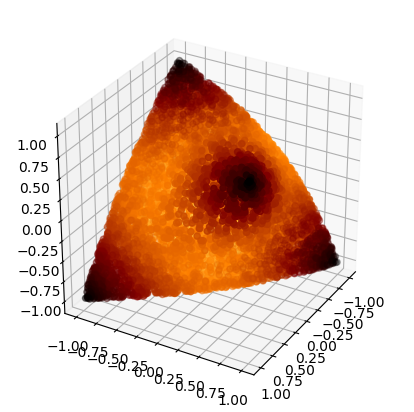
\includegraphics[width=.4\textwidth]{elliptope30}
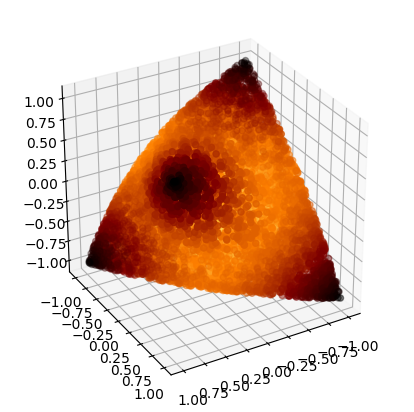
\includegraphics[width=.4\textwidth]{elliptope60}
\caption{The elliptope $\mathcal{C}_3$ (two different perspectives).}\label{fig:elliptope}
\end{figure}

In order to compute the Hilbert distance $\rho_{\mathrm{HG}}(C_1,C_2)$, we
need to compute the intersection of the line $(C_1,C_2)$ with 
$\partial\mathcal{C}$, denoted as $C_1'$ and $C_2'$, then we have
$$
\rho_{\mathrm{HG}}(C_1,C_2)=
\left\vert
\log\frac{\Vert{}C_1-C_2'\Vert \Vert{}C_1'-C_2\Vert}{\Vert{}C_1-C_1'\Vert \Vert{}C_2-C_2'\Vert}
\right\vert.
$$
Unfortunately there is no closed form solution of $C_1'$ and $C_2'$.
Instead, we apply a binary searching algorithm.
Note a necessary condition for $C\in\mathcal{C}$ is that $C$ has a positive spectrum.
If $C$ has at least one non-positive eigenvalue, then $C\notin\mathcal{C}$.
To determine whether a given $C$ is inside the elliptope requires a spectral
decomposition of $C$. Therefore the computation of $C_1'$ and $C_2'$ is in general expensive.

We compare the Hilbert elliptope geometry with commonly used distance measures
including the $L_2$ distance $\rho_{\mathrm{EUC}}$, $L_1$ distance $\rho_{\mathrm{L1}}$,
and the square root of the log-det divergence
$$
\rho_{\mathrm{LD}}(C_1,C_2) = tr(C_1C_2^{-1}) - \log\vert{}C_1C_2^{-1}\vert - d.
$$
Due to the high computational complexity, we only investigate $k$-means++ clustering.
The investigated dataset consists of 100 matrices forming 3 clusters in $\mathcal{C}_3$ with
almost identical size.  Each cluster is independently generated according to
\begin{align}
&P\sim \mathcal{W}^{-1}(I_{3\times{3}}, \nu_1),\nonumber\\
&C_i\sim \mathcal{W}^{-1}(P,\nu_2),\nonumber
\end{align}
where $\mathcal{W}^{-1}(A,\nu)$ denotes the inverse Wishart distribution with
scale matrix $A$ and $\nu$ degrees of freedom, and $C_i$ is a point in the cluster
associated with $P$.
Table \ref{tbl:elliptope} shows the $k$-means++ clustering performance in terms of NMI.
Again Hilbert geometry is favorable as compared to alternatives, showing
that the good performance of Hilbert clustering is generalizable.
\begin{table}[t]
\centering
\caption{NMI (mean$\pm$std) of $k$-means++ clustering based on different distance measures in the elliptope
(500 independent runs)}
\label{tbl:elliptope}
\begin{tabular}{cc|cccc}
\toprule[1.5pt]
$\nu_1$ & $\nu_2$    &  $\rho_{\mathrm{HG}}$ & $\rho_{\mathrm{EUC}}$ & $\rho_{\mathrm{L1}}$ & $\rho_{\mathrm{LD}}$ \\
\hline
$4$ & $10$ &  $\bm{0.62\pm0.22}$ & 0.57$\pm$0.21 & 0.56$\pm$0.22 & 0.58$\pm$0.22\\
$4$ & $30$ &  $\bm{0.85\pm0.18}$ & 0.80$\pm$0.20 & 0.81$\pm$0.19 & 0.82$\pm$0.20\\
$4$ & $50$ &  $\bm{0.89\pm0.17}$ & 0.87$\pm$0.17 & 0.86$\pm$0.18 & 0.88$\pm$0.18\\
\hline
$5$ & $10$ &  $\bm{0.50\pm0.21}$ & 0.49$\pm$0.21 & 0.48$\pm$0.20 & 0.47$\pm$0.21\\
$5$ & $30$ &  $\bm{0.77\pm0.20}$ & 0.75$\pm$0.21 & 0.75$\pm$0.21 & 0.75$\pm$0.21\\
$5$ & $50$ &  $\bm{0.84\pm0.19}$ & 0.82$\pm$0.19 & 0.82$\pm$0.20 & $\bm{0.84\pm0.18}$\\
\bottomrule[1.5pt]
\end{tabular}
\end{table}


%%%%%%%%%%%%%
\section{Conclusion}\label{sec:con}
%%%%%%%%%%%%

We introduced the Hilbert metric distance and its underlying non-Riemannian geometry
for modeling the space of multinomials or the open probability simplex.
We compared experimentally in simulated clustering tasks
this geometry with the traditional differential geometric modelings
(either FHR metric connection or dually coupled non-metric affine connections of information geometry \cite{IG-2016}).

The main feature of HG is that it is a metric non-manifold geometry, where geodesics are straight (Euclidean) line segments.
In simplex domains, the Hilbert balls have fixed combinatorial (Euclidean) polytope structures,
and HG is known to be isometric to a normed space~\cite{HilbertHarpe-1991,HilbertNormedSpace-2005}.
This latter isometry allows one to generalize easily the standard proofs of clustering ({\it e.g.}, $k$-means or $k$-center).
We demonstrated it for the $k$-means++ competitive performance analysis, and for the convergence of the $1$-center heuristic~\cite{bc-2003} (smallest enclosing Hilbert ball allows one to implement efficiently the $k$-center clustering).
Our experimental  $k$-means++ or $k$-center comparisons of HG algorithms with the  manifold modeling approach yield superior performance.
This may be intuitively explained by the sharpness of Hilbert balls as compared to the FHR/IG ball profiles.

Chentsov~\cite{cencov-2000} defined statistical invariance on a probability manifold under Markov morphisms, and proved that the Fisher Information Metric is the unique Riemannian metric (up to rescaling) for multinomials. However, this does not rule out that other distances (with underlying geometric structures) may be used to model statistical manifolds ({\it e.g.}, Finsler statistical manifolds~\cite{Cena-2002,FinslerIG-2016}, or the total variation distance --- the only metric $f$-divergence~\cite{L1metricfdiv-2007}). Defining statistical invariance related to geometry is the cornerstone problem of information geometry that can be tackled from many directions (see~\cite{statinvar-2017} and references therein for a short review). 

In this paper, we introduced Hilbert geometries in machine learning by considering clustering tasks in the probability simplex and in the elliptope.
Hilbert geometries proved computationally handy since geodesics are straight lines. 
One future direction is to consider the Hilbert metric for regularization and sparsity in machine learning (due to its equivalence with a polytope normed distance).
\vskip 0.5cm


\vbox{
Our Python codes are freely available online for reproducible research:\\
\centerline{\url{https://www.lix.polytechnique.fr/~nielsen/HSG/}}
}
%\subsection{Geometry and statistical invariance}
%
%We have described three geometries for modeling the open probability simplex $\Delta^d$: 
%$(\Delta^d,g)$, $(\Delta^d,\nabla^\alpha,\nabla^{-\alpha})$ and $\HG(\Delta^d)$.
%Geometry is concerned with invariance, and statistical spaces with statistical isomorphisms.
%Which geometry makes sense for modeling $\Delta^d$?
%Chensov~\cite{cencov-2000} considered statistical invariance of sufficient statistics under the Markov morphism of a random variable, and proved that
%for normed spaces, $\ell_1$ is the only norm that satisfies the invariance (with corresponding metric distance the total variation, see Theorem 6.3 of~\cite{cencov-2000}), and for differential geometry 
%the Fisher-Rao metric and $\alpha$-connections yield statistical invariance. 
%But this does not rule other kinds of appropriate geometries (like the Hilbert geometry).

%This paper focuses on comparing experimentally those three modelings.
%In particular, for HG, two balls can have infinitely many points of tangencies (share portion of an Euclidean edge).
%
%Note that the notion of ``statistical manifolds'' ({\em ie.}, DG with dual affine connections) is used beyond the scope of probability spaces.
%For example, one may use the statistical manifold modeling for studying the manifold of positive-definite matrices which play a role in control theory or linear programming, see~\cite{IG-2016}.

\bibliographystyle{spmpsci}
\bibliography{HilbertGeometryBIB}

\newpage
\appendix

%%%%%%%%%%%%%
\section{Isometry of Hilbert simplex geometry to a normed vector space\label{sec:isometry}}
%%%%%%%%%%%%%

Consider the Hilbert simplex metric space $(\Delta^d,\rho_\HG)$ where $\Delta^d$ denotes
the $d$-dimensional open probability simplex and $\rho_\HG$ the Hilbert cross-ratio metric.
Let us recall the isometry (\cite{HilbertHarpe-1991}, 1991) of the open standard simplex to a normed vector space $(V^d,\|\cdot\|_\NH)$. 
Let $V^d=\{v\in\bbR^{d+1} \st \sum_i v^i=0\}$ denote the $d$-dimensional vector space sitting in $\bbR^{d+1}$.
Map a point $p=(\lambda^0,\ldots,\lambda^{d})\in\Delta^d$ to a point $v(x)=(v^0,\ldots, v^{d})\in V^d$ as follows:
\begin{equation*}
v^i
= \frac{1}{d+1} \left(d\log \lambda^i -\sum_{j\neq{i}}\log \lambda^j \right)
= \log\lambda^i - \frac{1}{d+1}\sum_j \log\lambda^j.
\end{equation*}

We define the corresponding norm $\|\cdot\|_\NH$ in $V^d$ by considering the shape of its unit ball 
$B_V=\{v\in V^d \st |v^i-v^j|\leq 1, \forall i\not =j\}$.
The unit ball $B_V$ is a symmetric convex set containing the origin in its interior, and thus yields a {\em polytope norm}
 $\|\cdot\|_\NH$ (Hilbert norm) with $2\binom{d+1}{2}=d(d+1)$ facets.
Reciprocally, let us notice that a norm induces a unit ball centered at the origin that is convex and symmetric around the origin.

The distance in the normed vector space between $v\in V^d$ and $v'\in V^d$ is defined by:
\begin{equation*}
\rho_V(v,v')= \|v-v'\|_\NH = \inf \left\{ \tau \st v'\in \tau(B_V\oplus \{v\}) \right\},
\end{equation*}
where $A\oplus B=\{a+b \st a\in A,b\in B\}$ is the Minkowski sum.

The reverse map from the normed space $V^d$ to the probability simplex $\Delta^d$ is given by:
\begin{equation*}
\lambda^i = \frac{\exp({v^i})}{\sum_j \exp(v^j)}.
\end{equation*}


Thus we have $(\Delta^d,\rho_\HG)\cong (V^d,\|\cdot\|_\NH)$.
In 1D, $(V^1,\|\cdot\|_\NH)$ is isometric to the Euclidean line. 

Note that computing the distance in the normed vector space requires naively $O(d^2)$ time.

Unfortunately, the norm $\|\cdot\|_\NH$ does not satisfy the parallelogram law.\footnote{ Consider 
$A = (1/3,1/3,1/3)$, $B = (1/6,1/2,1/3)$, $C = (1/6,2/3,1/6)$ and
$D = (1/3,1/2,1/6)$. Then  $2AB^2 +2BC^2 = 4.34$ but $AC^2 + BD^2 = 3.84362411135$.
}
Notice that a norm satisfying the parallelogram law can be associated with an inner product via the polarization identity.
Thus the isometry of the Hilbert geometry to a normed vector space is not equipped with an inner product.
However, all norms in a finite dimensional space are equivalent.
This implies that in finite dimension, $(\Delta^d,\rho_\HG)$ is {\em quasi-isometric} to the Euclidean space $\bbR^d$.
An example of Hilbert geometry in infinite dimension is reported in~\cite{HilbertHarpe-1991}.
Hilbert spaces are not CAT spaces except when $\calC$ is an ellipsoid~\cite{Vernicos-2004}.

%%%%%%%%%%
\section{Hilbert geometry with Finslerian/Riemannian structures\label{sec:HGFG}}
%%%%%%%%%

In a Riemannian geometry, each tangent plane $T_pM$ of a $d$-dimensional manifold $M$ is equivalent to $\bbR^d$: $T_pM\simeq \bbR^d$.
The inner product at each tangent plane $T_pM$ can be visualized by an ellipsoid shape, a convex symmetric object centered at point $p$.
In a {\em Finslerian geometry},  a norm $\|\cdot\|_p$ is defined in each tangent plane $T_pM$, 
and this norm is visualized as a symmetric convex object with non-empty interior. 
Finslerian geometry thus generalizes Riemannian geometry by taking into account generic symmetric convex objects instead of ellipsoids for inducing norms at each tangent plane.
Any Hilbert geometry induced by a compact convex domain $\calC$ can be expressed by an equivalent Finslerian geometry by defining the norm in $T_p$ at $p$ as follows~\cite{Vernicos-2004}:

\begin{equation*}
\|v\|_p = F_\calC(p,v) =\frac{\|v\|}{2} \left( \frac{1}{pp^+} + \frac{1}{pp^-} \right),
\end{equation*}
where 
$F_\calC$ is the {\em Finsler metric},
$\|\cdot\|$ is an {\em arbitrary norm} on $\bbR^d$,
and $p^+$ and $p^-$ are the intersection points of the line passing through $p$ with direction $v$:
$$
p^+=p+t^+v,\quad p^-=p+t^-v.
$$


A geodesic $\gamma$ in a Finslerian geometry satisfies:
\begin{equation*}
d_\calC(\gamma(t_1),\gamma(t_2)) = \int_{t_1}^{t_2} F_\calC(\gamma(t),\dot\gamma(t)) \dt .
\end{equation*}

In $T_pM$, a ball of center $c$ and radius $r$ is defined by:
\begin{equation*}
B(c,r)=\{ v \ : \ F_\calC(c,v) \leq r \}.
\end{equation*}

Thus any Hilbert geometry induces an equivalent Finslerian geometry, and since Finslerian geometries include Riemannian geometries, one may wonder which Hilbert geometries induce Riemannian structures?
The only Riemannian geometries induced by Hilbert geometries are the {\em hyperbolic Cayley-Klein geometries}~\cite{Richter-2011,LMNN-2016,CayleyClassification-2016} with the domain $\calC$ being an ellipsoid.
The Finslerian modeling of information geometry has been studied in~\cite{Cena-2002,FinslerIG-2016}.

There is not a canonical way of defining measures in a Hilbert geometry since Hilbert geometries are Finslerian but not necessary Riemannian geometries~\cite{Vernicos-2004}. The Busemann measure is defined according to the Lebesgue measure $\lambda$ of $\bbR^d$: Let $B_p$ denote the unit ball wrt. to the Finsler norm at point $p\in\calC$, and $B_e$ the Euclidean unit ball. Then the Busemann measure for a Borel set $\calB$ is defined by~\cite{Vernicos-2004}:
$$
\mu_\calC(\calB) = \int_\calB \frac{\lambda(B_e)}{\lambda(B_p)} \mathrm{d}\lambda(p).
$$

The existence and uniqueness of center points of a probability measure in Finsler geometry have been investigated in~\cite{FinslerCenter-2012}.

%%%
\section{Bounding Hilbert norm with other norms}
%%%
Let us show that $\|v\|_\NH\leq \beta_{d,c} \|v\|_c$, where $\|\cdot\|_c$ 
is any norm.
Let $v=\sum_{i=0}^{d} e_i x_i$, where $\{e_i\}$ is a basis of $\bbR^{d+1}$.
We have:
$$
\|v\|_c \leq \sum_{i=0}^{d} |x_i|  \|e_i\|_c \leq \|x\|_2 
\underbrace{\sqrt{\sum_{i=0}^{d} \|e_i\|^2_c}}_{\beta_d},
$$
where the first inequality comes from the triangle inequality, and the 
second inequality is from the Cauchy-Schwarz inequality.
Thus we have:
$$
\|v\|_\NH \leq \beta_d \|x\|_2,
$$
with $\beta_d=\sqrt{d+1}$ since $\|e_i\|_\NH\leq 1$.

Let $\alpha_{d,c}=\min_{\{v \st \|v\|_c = 1\}} \|v\|_\NH$.
Consider $u=\frac{v}{\|v\|_c}$. Then $\|u\|_c=1$ so that $\|v\|_\NH\geq 
\alpha_{d,c} \|v\|_c$.
To find $\alpha_d$, we consider the unit $\ell_2$ ball in $V^d$, and 
find the smallest $\lambda>0$ so that
$\lambda B_V$ fully contains the Euclidean ball.

\begin{figure}[b]
\centering
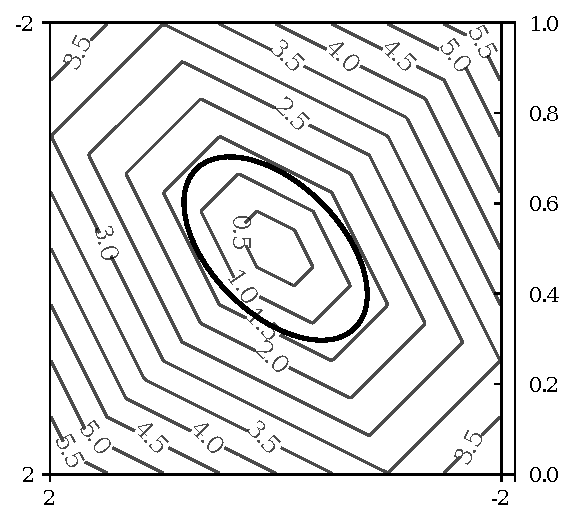
\includegraphics[width=.5\textwidth]{boundnorm}
\caption{Polytope balls $B_V$ and the Euclidean unit ball $B_E$.
From the figure the smallest polytope ball has radius $\approx1.5$.}
%$\alpha B_V$ enclosing $B_E$.}
\end{figure}

Therefore, we have overall:

$$
\alpha_d \|x\|_2 \leq \|v\|_\NH \leq \sqrt{d+1} \|x\|_2
$$

In general, note that we may consider two arbitrary norms $\|\cdot\|_l$ 
and $\|\cdot\|_u$ so that:
$$
\alpha_{d,l} \|x\|_l \leq \|v\|_\NH \leq \beta_{d,u} \|x\|_u.
$$

\section{Funk directed metrics and Funk balls}

The Funk metric~\cite{FunkHilbert-2014}
wrt a convex domain $\calC$ is defined by
$$
F_\calC(x,y) = \log\left( \frac{\|x-a\|}{\|y-a\|} \right),
$$
where $a$ is the intersection of 
the domain boundary and the affine ray $R(x,y)$
starting from $x$ and passing through $y$
Correspondingly, the reverse Funk metric is
$$
F_\calC(y,x) = \log\left( \frac{\|y-b\|}{\|x-b\|} \right),
$$
%with $b=r_\calC(y,x)$,
where $b$ is the intersection of $R(y,x)$ with the boundary.
The Funk metric is \emph{not} a metric distance.

The Hilbert metric is simply the arithmetic symmetrization:
$$
H_\calC(x,y)=\frac{F_\calC(x,y)+F_\calC(y,x)}{2}.
$$

It is interesting to explore clustering based on the Funk geometry,
which we leave as a future work.

%Forward ball is Euclidean a homothet of the domain of center $r$ and dilation factor $(1 - e^{-\rho})$ (cf. proposition 5.1, \cite{FunkHilbert-2014})

\end{document}
